% toolsoftrade/toolsoftrade.tex
% mainfile: ../perfbook.tex
% SPDX-License-Identifier: CC-BY-SA-3.0

\QuickQuizChapter{chp:Tools of the Trade}{Tools of the Trade}{qqztoolsoftrade}
%
\Epigraph{You are only as good as your tools, and your tools are only
	  as good as you are.}{\emph{Unknown}}

This chapter provides a brief introduction to some basic tools of the
parallel-programming trade, focusing mainly on those available to
user applications running on operating systems similar to Linux.
Section~\ref{sec:toolsoftrade:Scripting Languages} begins with
scripting languages,
Section~\ref{sec:toolsoftrade:POSIX Multiprocessing}
describes the multi-process parallelism supported by the POSIX API and
touches on POSIX threads,
Section~\ref{sec:toolsoftrade:Alternatives to POSIX Operations}
presents analogous operations in other environments, and finally,
Section~\ref{sec:toolsoftrade:The Right Tool for the Job: How to Choose?}
helps to choose the tool that will get the job done.

\QuickQuiz{
	You call these tools???
	They look more like low-level synchronization primitives to me!
}\QuickQuizAnswer{
	They look that way because they are in fact low-level synchronization
	primitives.
	And they are in fact the fundamental tools for building low-level
	concurrent software.
}\QuickQuizEnd

Please note that this chapter provides but a brief introduction.
More detail is available from the references (and from the Internet),
and more information will be provided in later chapters.

\section{Scripting Languages}
\label{sec:toolsoftrade:Scripting Languages}
%
\epigraph{The supreme excellence is simplicity.}
	 {\emph{Henry Wadsworth Longfellow, abbreviated}}

The Linux shell scripting languages provide simple but effective ways
of managing parallelism.
For example, suppose that you had a program \co{compute_it}
that you needed to run twice with two different sets of arguments.
This can be accomplished using UNIX shell scripting as follows:

\input{CodeSamples/toolsoftrade/parallel@compute_it.fcv}

\begin{figure}[tb]
\centering
\resizebox{3in}{!}{\includegraphics{toolsoftrade/shellparallel}}
\caption{Execution Diagram for Parallel Shell Execution}
\label{fig:toolsoftrade:Execution Diagram for Parallel Shell Execution}
\end{figure}

\begin{fcvref}[ln:toolsoftrade:parallel:compute_it]
Lines~\lnref{comp1} and~\lnref{comp2} launch two instances of this
program, redirecting their
output to two separate files, with the \co{&} character directing the
shell to run the two instances of the program in the background.
Line~\lnref{wait} waits for both instances to complete, and
lines~\lnref{cat1} and~\lnref{cat2}
display their output.
\end{fcvref}
The resulting execution is as shown in
Figure~\ref{fig:toolsoftrade:Execution Diagram for Parallel Shell Execution}:
the two instances of \co{compute_it} execute in parallel,
\co{wait} completes after both of them do, and then the two instances
of \co{cat} execute sequentially.
% @@@ Maui scheduler, load balancing, BOINC, and so on.
% @@@ Diagram showing parallel execution.

\QuickQuizSeries{%
\QuickQuizB{
	But this silly shell script isn't a \emph{real} parallel program!
	Why bother with such trivia???
}\QuickQuizAnswerB{
	Because you should \emph{never} forget the simple stuff!

	Please keep in mind that the title of this book is
	``Is Parallel Programming Hard, And, If So, What Can You Do About It?''.
	One of the most effective things you can do about it is to
	avoid forgetting the simple stuff!
	After all, if you choose to do parallel programming the hard
	way, you have no one but yourself to blame.
}\QuickQuizEndB
%
\QuickQuizE{
	Is there a simpler way to create a parallel shell script?
	If so, how?  If not, why not?
}\QuickQuizAnswerE{
	One straightforward approach is the shell pipeline:

\begin{VerbatimU}
grep $pattern1 | sed -e 's/a/b/' | sort
\end{VerbatimU}

	For a sufficiently large input file,
	\co{grep} will pattern-match in parallel with \co{sed}
	editing and with the input processing of \co{sort}.
	See the file \path{parallel.sh} for a demonstration of
	shell-script parallelism and pipelining.
}\QuickQuizEndE
}

For another example, the \co{make} software-build scripting language
provides a \co{-j} option that specifies how much parallelism should be
introduced into the build process.
Thus, typing \co{make -j4} when building a Linux kernel specifies that
up to four build steps be executed concurrently.

It is hoped that these simple examples convince you that parallel
programming need not always be complex or difficult.

\QuickQuiz{
	But if script-based parallel programming is so easy, why
	bother with anything else?
}\QuickQuizAnswer{
	In fact, it is quite likely that a very large fraction of
	parallel programs in use today are script-based.
	However, script-based parallelism does have its limitations:
	\begin{enumerate}
	\item	Creation of new processes is usually quite heavyweight,
		involving the expensive \co{fork()} and \co{exec()}
		system calls.
	\item	Sharing of data, including pipelining, typically involves
		expensive file I/O.
	\item	The reliable synchronization primitives available to
		scripts also typically involve expensive file I/O.
	\item	Scripting languages are often too slow, but are often
		quite useful when coordinating execution of long-running
		programs written in lower-level programming languages.
	\end{enumerate}
	These limitations require that script-based parallelism use
	coarse-grained parallelism, with each unit of work having
	execution time of at least tens of milliseconds, and preferably
	much longer.

	Those requiring finer-grained parallelism are well advised to
	think hard about their problem to see if it can be expressed
	in a coarse-grained form.
	If not, they should consider using other parallel-programming
	environments, such as those discussed in
	Section~\ref{sec:toolsoftrade:POSIX Multiprocessing}.
}\QuickQuizEnd

\section{POSIX Multiprocessing}
\label{sec:toolsoftrade:POSIX Multiprocessing}
%
\epigraph{A camel is a horse designed by committee.}{\emph{Unknown}}

This section scratches the surface of the
POSIX environment, including pthreads~\cite{OpenGroup1997pthreads},
as this environment is readily available and widely implemented.
Section~\ref{sec:toolsoftrade:POSIX Process Creation and Destruction}
provides a glimpse of the POSIX \co{fork()} and related primitives,
Section~\ref{sec:toolsoftrade:POSIX Thread Creation and Destruction}
touches on thread creation and destruction,
Section~\ref{sec:toolsoftrade:POSIX Locking} gives a brief overview
of POSIX locking, and, finally,
Section~\ref{sec:toolsoftrade:POSIX Reader-Writer Locking} describes a
specific lock which can be used for data that is read by many threads and only
occasionally updated.

\subsection{POSIX Process Creation and Destruction}
\label{sec:toolsoftrade:POSIX Process Creation and Destruction}

Processes are created using the \apipx{fork()} primitive, they may
be destroyed using the \apipx{kill()} primitive, they may destroy
themselves using the \apipx{exit()} primitive.
A process executing a \co{fork()} primitive is said to be the ``parent''
of the newly created process.
A parent may wait on its children using the \apipx{wait()} primitive.

Please note that the examples in this section are quite simple.
Real-world applications using these primitives might need to manipulate
signals, file descriptors, shared memory segments, and any number of
other resources.
In addition, some applications need to take specific actions if a given
child terminates, and might also need to be concerned with the reason
that the child terminated.
These issues can of course add substantial complexity to the code.
For more information, see any of a number of textbooks on the
subject~\cite{WRichardStevens1992,StewartWeiss2013UNIX}.

\begin{listing}[tbp]
\begin{fcvlabel}[ln:toolsoftrade:forkjoin:main]
\begin{VerbatimL}[commandchars=\%\[\]]
pid = fork();%lnlbl[fork]
if (pid == 0) {%lnlbl[if]
	/* child */%lnlbl[child]
} else if (pid < 0) {%lnlbl[else]
	/* parent, upon error */%lnlbl[errora]
	perror("fork");
	exit(EXIT_FAILURE);%lnlbl[errorb]
} else {
	/* parent, pid == child ID */%lnlbl[parent]
}
\end{VerbatimL}
\end{fcvlabel}
\caption{Using the \tco{fork()} Primitive}
\label{lst:toolsoftrade:Using the fork() Primitive}
\end{listing}

\begin{fcvref}[ln:toolsoftrade:forkjoin:main]
If \co{fork()} succeeds, it returns twice, once for the parent
and again for the child.
The value returned from \co{fork()} allows the caller to tell
the difference, as shown in
Listing~\ref{lst:toolsoftrade:Using the fork() Primitive}
(\path{forkjoin.c}).
Line~\lnref{fork} executes the \co{fork()} primitive, and saves
its return value in local variable \co{pid}.
Line~\lnref{if} checks to see if \co{pid} is zero, in which case,
this is the child, which continues on to execute line~\lnref{child}.
As noted earlier, the child may terminate via the \co{exit()} primitive.
Otherwise, this is the parent, which checks for an error return from
the \co{fork()} primitive on line~\lnref{else}, and prints an error
and exits on \clnrefrange{errora}{errorb} if so.
Otherwise, the \co{fork()} has executed successfully, and the parent
therefore executes line~\lnref{parent} with the variable \co{pid}
containing the process ID of the child.
\end{fcvref}

\begin{listing}[tbp]
\input{CodeSamples/api-pthreads/api-pthreads@waitall.fcv}
\caption{Using the \tco{wait()} Primitive}
\label{lst:toolsoftrade:Using the wait() Primitive}
\end{listing}

\begin{fcvref}[ln:api-pthreads:api-pthreads:waitall]
The parent process may use the \apipx{wait()} primitive to wait for its children
to complete.
However, use of this primitive is a bit more complicated than its shell-script
counterpart, as each invocation of \co{wait()} waits for but one child
process.
It is therefore customary to wrap \co{wait()} into a function similar
to the \apipx{waitall()} function shown in
Listing~\ref{lst:toolsoftrade:Using the wait() Primitive}
(\path{api-pthreads.h}),
with this \co{waitall()} function having semantics similar to the
shell-script \co{wait} command.
Each pass through the loop spanning \clnrefrange{loopa}{loopb}
waits on one child process.
Line~\lnref{wait} invokes the \co{wait()} primitive, which blocks
until a child process exits, and returns that child's process ID.
If the process ID is instead $-1$, this indicates that the \co{wait()}
primitive was unable to wait on a child.
If so, line~\lnref{ECHILD} checks for the \co{ECHILD} errno, which
indicates that there are no more child processes, so that
line~\lnref{break} exits the loop.
Otherwise, lines~\lnref{perror} and~\lnref{exit} print an error and exit.
\end{fcvref}

\QuickQuiz{
	Why does this \co{wait()} primitive need to be so complicated?
	Why not just make it work like the shell-script \co{wait} does?
}\QuickQuizAnswer{
	Some parallel applications need to take special action when
	specific children exit, and therefore need to wait for each
	child individually.
	In addition, some parallel applications need to detect the
	reason that the child died.
	As we saw in Listing~\ref{lst:toolsoftrade:Using the wait() Primitive},
	it is not hard to build a \co{waitall()} function out of
	the \co{wait()} function, but it would be impossible to
	do the reverse.
	Once the information about a specific child is lost, it is lost.
}\QuickQuizEnd

\begin{listing}[tbp]
\input{CodeSamples/toolsoftrade/forkjoinvar@main.fcv}
\caption{Processes Created Via \tco{fork()} Do Not Share Memory}
\label{lst:toolsoftrade:Processes Created Via fork() Do Not Share Memory}
\end{listing}

\begin{fcvref}[ln:toolsoftrade:forkjoinvar:main]
It is critically important to note that the parent and child do \emph{not}
share memory.
This is illustrated by the program shown in
Listing~\ref{lst:toolsoftrade:Processes Created Via fork() Do Not Share Memory}
(\path{forkjoinvar.c}),
in which the child sets a global variable \co{x} to 1 on line~\lnref{setx},
prints a message on line~\lnref{print:c}, and exits on line~\lnref{exit:s}.
The parent continues at line~\lnref{waitall}, where it waits on the child,
and on line~\lnref{print:p} finds that its copy of the variable \co{x} is
still zero. The output is thus as follows:
\end{fcvref}

\begin{VerbatimU}
Child process set x=1
Parent process sees x=0
\end{VerbatimU}

\QuickQuiz{
	Isn't there a lot more to \co{fork()} and \co{wait()}
	than discussed here?
}\QuickQuizAnswer{
	Indeed there is, and
	it is quite possible that this section will be expanded in
	future versions to include messaging features (such as UNIX
	pipes, TCP/IP, and shared file I/O) and memory mapping
	(such as \co{mmap()} and \co{shmget()}).
	In the meantime, there are any number of textbooks that cover
	these primitives in great detail,
	and the truly motivated can read manpages, existing parallel
	applications using these primitives, as well as the
	source code of the Linux-kernel implementations themselves.

	It is important to note that the parent process in
	Listing~\ref{lst:toolsoftrade:Processes Created Via fork() Do Not Share Memory}
	waits until after the child terminates to do its \co{printf()}.
	Using \co{printf()}'s buffered I/O concurrently to the same file
	from multiple processes is non-trivial, and is best avoided.
	If you really need to do concurrent buffered I/O,
	consult the documentation for your OS.
	For UNIX/Linux systems, Stewart Weiss's lecture notes provide
	a good introduction with informative
	examples~\cite{StewartWeiss2013UNIX}.
}\QuickQuizEnd

The finest-grained parallelism requires shared memory, and
this is covered in
Section~\ref{sec:toolsoftrade:POSIX Thread Creation and Destruction}.
That said, shared-memory parallelism can be significantly more complex
than fork-join parallelism.

\subsection{POSIX Thread Creation and Destruction}
\label{sec:toolsoftrade:POSIX Thread Creation and Destruction}

\begin{fcvref}[ln:toolsoftrade:pcreate:mythread]
To create a thread within an existing process, invoke the
\apipx{pthread_create()} primitive, for example, as shown on
lines~\lnref{create:a} and~\lnref{create:b} of
Listing~\ref{lst:toolsoftrade:Threads Created Via pthread-create() Share Memory}
(\path{pcreate.c}).
The first argument is a pointer to a \co{pthread_t} in which to store the
ID of the thread to be created, the second \co{NULL} argument is a pointer
to an optional \co{pthread_attr_t}, the third argument is the function
(in this case, \co{mythread()})
that is to be invoked by the new thread, and the last \co{NULL} argument
is the argument that will be passed to \co{mythread}.
\end{fcvref}

\begin{listing}[tbp]
\input{CodeSamples/toolsoftrade/pcreate@mythread.fcv}
\caption{Threads Created Via \tco{pthread_create()} Share Memory}
\label{lst:toolsoftrade:Threads Created Via pthread-create() Share Memory}
\end{listing}

In this example, \co{mythread()} simply returns, but it could instead
call \apipx{pthread_exit()}.

\QuickQuiz{
	If the \co{mythread()} function in
	Listing~\ref{lst:toolsoftrade:Threads Created Via pthread-create() Share Memory}
	can simply return, why bother with \co{pthread_exit()}?
}\QuickQuizAnswer{
	In this simple example, there is no reason whatsoever.
	However, imagine a more complex example, where \co{mythread()}
	invokes other functions, possibly separately compiled.
	In such a case, \co{pthread_exit()} allows these other functions
	to end the thread's execution without having to pass some sort
	of error return all the way back up to \co{mythread()}.
}\QuickQuizEnd

\begin{fcvref}[ln:toolsoftrade:pcreate:mythread]
The \apipx{pthread_join()} primitive, shown on line~\lnref{join},
is analogous to
the fork-join \apipx{wait()} primitive.
It blocks until the thread specified by the \co{tid} variable completes
execution, either by invoking \apipx{pthread_exit()} or by returning from
the thread's top-level function.
The thread's exit value will be stored through the pointer passed as the
second argument to \co{pthread_join()}.
The thread's exit value is either the value passed to \co{pthread_exit()}
or the value returned by the thread's top-level function, depending on
how the thread in question exits.
\end{fcvref}

The program shown in
Listing~\ref{lst:toolsoftrade:Threads Created Via pthread-create() Share Memory}
produces output as follows, demonstrating that memory is in fact
shared between the two threads:

\begin{VerbatimU}
Child process set x=1
Parent process sees x=1
\end{VerbatimU}

Note that this program carefully makes sure that only one of the threads
stores a value to variable \co{x} at a time.
Any situation in which one thread might be storing a value to a given
variable while some other thread either loads from or stores to that
same variable is termed a ``data race''.
Because the C language makes no guarantee that the results of a data race
will be in any way reasonable, we need some way of safely accessing
and modifying data concurrently, such as the locking primitives discussed
in the following section.

\QuickQuiz{
	If the C language makes no guarantees in presence of a data
	race, then why does the Linux kernel have so many data races?
	Are you trying to tell me that the Linux kernel is completely
	broken???
}\QuickQuizAnswer{
	Ah, but the Linux kernel is written in a carefully selected
	superset of the C language that includes special GNU
	extensions, such as asms, that permit safe execution even
	in presence of data races.
	In addition, the Linux kernel does not run on a number of
	platforms where data races would be especially problematic.
	For an example, consider embedded systems with 32-bit pointers
	and 16-bit busses.
	On such a system, a data race involving a store to and a load
	from a given pointer might well result in the load returning the
	low-order 16 bits of the old value of the pointer concatenated
	with the high-order 16 bits of the new value of the pointer.

	Nevertheless, even in the Linux kernel, data races can be
	quite dangerous and should be avoided where
	feasible~\cite{JonCorbet2012ACCESS:ONCE}.
}\QuickQuizEnd

\subsection{POSIX Locking}
\label{sec:toolsoftrade:POSIX Locking}

The POSIX standard allows the programmer to avoid data races via
``POSIX locking''.
POSIX locking features a number of primitives, the most fundamental
of which are \apipx{pthread_mutex_lock()} and \apipx{pthread_mutex_unlock()}.
These primitives operate on locks, which are of type \apipx{pthread_mutex_t}.
These locks may be declared statically and initialized with
\apipx{PTHREAD_MUTEX_INITIALIZER}, or they may be allocated dynamically
and initialized using the \apipx{pthread_mutex_init()} primitive.
The demonstration code in this section will take the former course.

The \co{pthread_mutex_lock()} primitive ``acquires'' the specified lock,
and the \co{pthread_mutex_unlock()} ``releases'' the specified lock.
Because these are ``exclusive'' locking primitives,
only one thread at a time may ``hold'' a given lock at a given time.
For example, if a pair of threads attempt to acquire the same lock
concurrently, one of the pair will be ``granted'' the lock first, and
the other will wait until the first thread releases the lock.
A simple and reasonably useful programming model permits a given data item
to be accessed only while holding the corresponding
lock~\cite{Hoare74}.

\QuickQuiz{
	What if I want several threads to hold the same lock at the
	same time?
}\QuickQuizAnswer{
	The first thing you should do is to ask yourself why you would
	want to do such a thing.
	If the answer is ``because I have a lot of data that is read
	by many threads, and only occasionally updated'', then
	POSIX reader-writer locks might be what you are looking for.
	These are introduced in
	Section~\ref{sec:toolsoftrade:POSIX Reader-Writer Locking}.

	Another way to get the effect of multiple threads holding
	the same lock is for one thread to acquire the lock, and
	then use \co{pthread_create()} to create the other threads.
	The question of why this would ever be a good idea is left
	to the reader.
}\QuickQuizEnd

\begin{listing}[tbp]
\input{CodeSamples/toolsoftrade/lock@reader_writer.fcv}
\caption{Demonstration of Exclusive Locks}
\label{lst:toolsoftrade:Demonstration of Exclusive Locks}
\end{listing}

\begin{fcvref}[ln:toolsoftrade:lock:reader_writer]
This exclusive-locking property is demonstrated using the code shown in
Listing~\ref{lst:toolsoftrade:Demonstration of Exclusive Locks}
(\path{lock.c}).
Line~\lnref{lock_a} defines and initializes a POSIX lock named \co{lock_a}, while
line~\lnref{lock_b} similarly defines and initializes a lock named \co{lock_b}.
Line~\lnref{x} defines and initializes a shared variable~\co{x}.
\end{fcvref}

\begin{fcvref}[ln:toolsoftrade:lock:reader_writer:reader]
\Clnrefrange{b}{e} define a function \co{lock_reader()} which repeatedly
reads the shared variable \co{x} while holding
the lock specified by \co{arg}.
Line~\lnref{cast} casts \co{arg} to a pointer to a \co{pthread_mutex_t}, as
required by the \co{pthread_mutex_lock()} and \co{pthread_mutex_unlock()}
primitives.
\end{fcvref}

\QuickQuizSeries{%
\QuickQuizB{
	Why not simply make the argument to \co{lock_reader()}
	on line~\ref{ln:toolsoftrade:lock:reader_writer:reader:b} of
	Listing~\ref{lst:toolsoftrade:Demonstration of Exclusive Locks}
	be a pointer to a \co{pthread_mutex_t}?
}\QuickQuizAnswerB{
	Because we will need to pass \co{lock_reader()} to
	\co{pthread_create()}.
	Although we could cast the function when passing it to
	\co{pthread_create()}, function casts are quite a bit
	uglier and harder to get right than are simple pointer casts.
}\QuickQuizEndB
%
\QuickQuizE{
	\begin{fcvref}[ln:toolsoftrade:lock:reader_writer]
	What is the \apik{READ_ONCE()} on
        lines~\lnref{reader:read_x} and~\lnref{writer:inc} and the
	\apik{WRITE_ONCE()} on line~\lnref{writer:inc} of
	Listing~\ref{lst:toolsoftrade:Demonstration of Exclusive Locks}?
	\end{fcvref}
}\QuickQuizAnswerE{
	These macros constrain the compiler so as to prevent it from
	carrying out optimizations that would be problematic for concurrently
	accessed shared variables.
	They don't constrain the CPU at all, other than by preventing
	reordering of accesses to a given single variable.
	Note that this single-variable constraint does apply to the
	code shown in
	Listing~\ref{lst:toolsoftrade:Demonstration of Exclusive Locks}
	because only the variable \co{x} is accessed.

	For more information on \co{READ_ONCE()} and \co{WRITE_ONCE()},
	please see
	Section~\ref{sec:toolsoftrade:Atomic Operations (gcc Classic)}.
	For more information on ordering accesses to multiple variables
	by multiple threads, please see
	Chapter~\ref{chp:Advanced Synchronization: Memory Ordering}.
	In the meantime, \co{READ_ONCE(x)} has much in common with
	the \GCC\  intrinsic \co{__atomic_load_n(&x, __ATOMIC_RELAXED)}
	and \co{WRITE_ONCE()} has much in common with the \GCC\ 
	intrinsic \co{__atomic_store_n(&x, v, __ATOMIC_RELAXED)}.
}\QuickQuizEndE
}

\begin{fcvref}[ln:toolsoftrade:lock:reader_writer:reader]
\Clnrefrange{acq:b}{acq:e} acquire the specified
\co{pthread_mutex_t}, checking
for errors and exiting the program if any occur.
\Clnrefrange{loop:b}{loop:e} repeatedly check the value of \co{x},
printing the new value
each time that it changes.
Line~\lnref{sleep} sleeps for one millisecond, which allows this demonstration
to run nicely on a uniprocessor machine.
\Clnrefrange{rel:b}{rel:e} release the \co{pthread_mutex_t},
again checking for
errors and exiting the program if any occur.
Finally, line~\lnref{return} returns \co{NULL}, again to match the function type
required by \co{pthread_create()}.
\end{fcvref}

\QuickQuiz{
	Writing four lines of code for each acquisition and release
	of a \co{pthread_mutex_t} sure seems painful!
	Isn't there a better way?
}\QuickQuizAnswer{
	Indeed!
	And for that reason, the \co{pthread_mutex_lock()} and
	\co{pthread_mutex_unlock()} primitives are normally wrapped
	in functions that do this error checking.
	Later on, we will wrap them with the Linux kernel
	\co{spin_lock()} and \co{spin_unlock()} APIs.
}\QuickQuizEnd

\begin{fcvref}[ln:toolsoftrade:lock:reader_writer:writer]
\Clnrefrange{b}{e} of
Listing~\ref{lst:toolsoftrade:Demonstration of Exclusive Locks}
show \co{lock_writer()}, which
periodically updates the shared variable \co{x} while holding the
specified \co{pthread_mutex_t}.
As with \co{lock_reader()}, line~\lnref{cast} casts \co{arg} to a pointer
to \co{pthread_mutex_t},
\clnrefrange{acq:b}{acq:e} acquire the specified lock,
and \clnrefrange{rel:b}{rel:e} release it.
While holding the lock, \clnrefrange{loop:b}{loop:e}
increment the shared variable \co{x},
sleeping for five milliseconds between each increment.
Finally, \clnrefrange{rel:b}{rel:e} release the lock.
\end{fcvref}

\begin{listing}[tbp]
\input{CodeSamples/toolsoftrade/lock@same_lock.fcv}
\caption{Demonstration of Same Exclusive Lock}
\label{lst:toolsoftrade:Demonstration of Same Exclusive Lock}
\end{listing}

\begin{fcvref}[ln:toolsoftrade:lock:same_lock]
Listing~\ref{lst:toolsoftrade:Demonstration of Same Exclusive Lock}
shows a code fragment that runs \co{lock_reader()} and
\co{lock_writer()} as threads using the same lock, namely, \co{lock_a}.
\Clnrefrange{cr:reader:b}{cr:reader:e} create a thread
running \co{lock_reader()}, and then
\clnrefrange{cr:writer:b}{cr:writer:e} create a thread
running \co{lock_writer()}.
\Clnrefrange{wait:b}{wait:e} wait for both threads to complete.
The output of this code fragment is as follows:
\end{fcvref}

\begin{VerbatimU}
Creating two threads using same lock:
lock_reader(): x = 0
\end{VerbatimU}

Because both threads are using the same lock, the \co{lock_reader()}
thread cannot see any of the intermediate values of \co{x} produced
by \co{lock_writer()} while holding the lock.

\QuickQuiz{
	Is ``x = 0'' the only possible output from the code fragment
	shown in
	Listing~\ref{lst:toolsoftrade:Demonstration of Same Exclusive Lock}?
	If so, why?
	If not, what other output could appear, and why?
}\QuickQuizAnswer{
	No.
	The reason that ``x = 0'' was output was that \co{lock_reader()}
	acquired the lock first.
	Had \co{lock_writer()} instead acquired the lock first, then
	the output would have been \mbox{``x = 3''}.
	However, because the code fragment started \co{lock_reader()} first
	and because this run was performed on a multiprocessor,
	one would normally expect \co{lock_reader()} to acquire the
	lock first.
	Nevertheless, there are no guarantees, especially on a busy system.
}\QuickQuizEnd

\begin{listing}[tbp]
\input{CodeSamples/toolsoftrade/lock@diff_lock.fcv}
\caption{Demonstration of Different Exclusive Locks}
\label{lst:toolsoftrade:Demonstration of Different Exclusive Locks}
\end{listing}

Listing~\ref{lst:toolsoftrade:Demonstration of Different Exclusive Locks}
shows a similar code fragment, but this time using different locks:
\co{lock_a} for \co{lock_reader()} and \co{lock_b} for
\co{lock_writer()}.
The output of this code fragment is as follows:

\begin{VerbatimU}
Creating two threads w/different locks:
lock_reader(): x = 0
lock_reader(): x = 1
lock_reader(): x = 2
lock_reader(): x = 3
\end{VerbatimU}

Because the two threads are using different locks, they do not exclude
each other, and can run concurrently.
The \co{lock_reader()} function can therefore see the intermediate
values of \co{x} stored by \co{lock_writer()}.

\QuickQuizSeries{%
\QuickQuizB{
	Using different locks could cause quite a bit of confusion,
	what with threads seeing each others' intermediate states.
	So should well-written parallel programs restrict themselves
	to using a single lock in order to avoid this kind of confusion?
}\QuickQuizAnswerB{
	Although it is sometimes possible to write a program using a
	single global lock that both performs and scales well, such
	programs are exceptions to the rule.
	You will normally need to use multiple locks to attain good
	performance and scalability.

	One possible exception to this rule is ``transactional memory'',
	which is currently a research topic.
	Transactional\-/memory semantics can be loosely thought of as those
	of a single global lock with optimizations permitted and
	with the addition of rollback~\cite{HansJBoehm2009HOTPAR}.
}\QuickQuizEndB
%
\QuickQuizM{
	In the code shown in
	Listing~\ref{lst:toolsoftrade:Demonstration of Different Exclusive Locks},
	is \co{lock_reader()} guaranteed to see all the values produced
	by \co{lock_writer()}?
	Why or why not?
}\QuickQuizAnswerM{
	No.
	On a busy system, \co{lock_reader()} might be preempted
	for the entire duration of \co{lock_writer()}'s execution,
	in which case it would not see \emph{any} of \co{lock_writer()}'s
	intermediate states for \co{x}.
}\QuickQuizEndM
%
\QuickQuizE{
	Wait a minute here!!!
	Listing~\ref{lst:toolsoftrade:Demonstration of Same Exclusive Lock}
	didn't initialize shared variable~\co{x},
	so why does it need to be initialized in
	Listing~\ref{lst:toolsoftrade:Demonstration of Different Exclusive Locks}?
}\QuickQuizAnswerE{
	See line~\ref{ln:toolsoftrade:lock:reader_writer:x} of
	Listing~\ref{lst:toolsoftrade:Demonstration of Exclusive Locks}.
	Because the code in
	Listing~\ref{lst:toolsoftrade:Demonstration of Same Exclusive Lock}
	ran first, it could rely on the compile-time initialization of~\co{x}.
	The code in
	Listing~\ref{lst:toolsoftrade:Demonstration of Different Exclusive Locks}
	ran next, so it had to re-initialize~\co{x}.
}\QuickQuizEndE
}

Although there is quite a bit more to POSIX exclusive locking, these
primitives provide a good start and are in fact sufficient in a great
many situations.
The next section takes a brief look at POSIX reader-writer locking.

\subsection{POSIX Reader-Writer Locking}
\label{sec:toolsoftrade:POSIX Reader-Writer Locking}

The POSIX API provides a reader-writer lock, which is represented by
a \apipx{pthread_rwlock_t}.
As with \apipx{pthread_mutex_t}, \co{pthread_rwlock_t} may be statically
initialized via \apipx{PTHREAD_RWLOCK_INITIALIZER} or dynamically
initialized via the \apipx{pthread_rwlock_init()} primitive.
The \apipx{pthread_rwlock_rdlock()} primitive read-acquires the
specified \apipx{pthread_rwlock_t}, the \apipx{pthread_rwlock_wrlock()}
primitive write-acquires it, and the \apipx{pthread_rwlock_unlock()}
primitive releases it.
Only a single thread may write-hold a given \apipx{pthread_rwlock_t}
at any given time, but multiple threads may read-hold a given
\apipx{pthread_rwlock_t}, at least while there is no thread
currently write-holding it.

As you might expect, reader-writer locks are designed for read-mostly
situations.
In these situations, a reader-writer lock can provide greater scalability
than can an exclusive lock because the exclusive lock is by definition
limited to a single thread holding the lock at any given time, while
the reader-writer lock permits
an arbitrarily large number of readers to concurrently hold the lock.
However, in practice, we need to know how much additional scalability is
provided by reader-writer locks.

\begin{listing}[tbp]
\input{CodeSamples/toolsoftrade/rwlockscale@reader.fcv}
\caption{Measuring Reader-Writer Lock Scalability}
\label{lst:toolsoftrade:Measuring Reader-Writer Lock Scalability}
\end{listing}

\begin{fcvref}[ln:toolsoftrade:rwlockscale:reader]
Listing~\ref{lst:toolsoftrade:Measuring Reader-Writer Lock Scalability}
(\path{rwlockscale.c})
shows one way of measuring reader-writer lock scalability.
Line~\lnref{rwlock} shows the definition and initialization of the reader-writer
lock, line~\lnref{holdtm} shows the \co{holdtime} argument controlling the
time each thread holds the reader-writer lock,
line~\lnref{thinktm} shows the \co{thinktime} argument controlling the time between
the release of the reader-writer lock and the next acquisition,
line~\lnref{rdcnts} defines the \co{readcounts} array into which each reader thread
places the number of times it acquired the lock, and
line~\lnref{nrdrun} defines the \co{nreadersrunning} variable, which
determines when all reader threads have started running.

\Clnrefrange{goflag:b}{goflag:e} define \co{goflag},
which synchronizes the start and the
end of the test.
This variable is initially set to \co{GOFLAG_INIT}, then set to
\co{GOFLAG_RUN} after all the reader threads have started, and finally
set to \co{GOFLAG_STOP} to terminate the test run.
\end{fcvref}

\begin{fcvref}[ln:toolsoftrade:rwlockscale:reader:reader]
\Clnrefrange{b}{e} define \co{reader()}, which is the reader thread.
Line~\lnref{atmc_inc} atomically increments the \co{nreadersrunning} variable
to indicate that this thread is now running, and
\clnrefrange{wait:b}{wait:e} wait for the test to start.
The \apik{READ_ONCE()} primitive forces the compiler to fetch \co{goflag}
on each pass through the loop---the compiler would otherwise be within its
rights to assume that the value of \co{goflag} would never change.
\end{fcvref}

\QuickQuizSeries{%
\QuickQuizB{
	Instead of using \apik{READ_ONCE()} everywhere, why not just
	declare \co{goflag} as \co{volatile} on
        line~\ref{ln:toolsoftrade:rwlockscale:reader:goflag:e} of
	Listing~\ref{lst:toolsoftrade:Measuring Reader-Writer Lock Scalability}?
}\QuickQuizAnswerB{
	A \co{volatile} declaration is in fact a reasonable alternative in
	this particular case.
	However, use of \apik{READ_ONCE()} has the benefit of clearly
	flagging to the reader that \co{goflag} is subject to concurrent
	reads and updates.
	Note that \apik{READ_ONCE()} is especially useful in cases where
	most of the accesses are protected by a lock (and thus \emph{not}
	subject to change), but where a few of the accesses are made outside
	of the lock.
	Using a volatile declaration in this case would make it harder
	for the reader to note the special accesses outside of the lock,
	and would also make it harder for the compiler to generate good
	code under the lock.
}\QuickQuizEndB
%
\QuickQuizM{
	\apik{READ_ONCE()} only affects the compiler, not the CPU.
	Don't we also need memory barriers to make sure
	that the change in \co{goflag}'s value propagates to the
	CPU in a timely fashion in
	Listing~\ref{lst:toolsoftrade:Measuring Reader-Writer Lock Scalability}?
}\QuickQuizAnswerM{
	No, memory barriers are not needed and won't help here.
	Memory barriers only enforce ordering among multiple memory
	references:  They absolutely do not guarantee to expedite the
	propagation of data from one part of the system to another.\footnote{
		There have been persistent rumors of hardware in which
		memory barriers actually do expedite propagation of data,
		but no confirmed sightings.}
	This leads to a quick rule of thumb:  You do not need
	memory barriers unless you are using more than one
	variable to communicate between multiple threads.

	But what about \co{nreadersrunning}?
	Isn't that a second variable used for communication?
	Indeed it is, and there really are the needed memory-barrier
	instructions buried in \apig{__sync_fetch_and_add()},
	which make sure that the thread proclaims its presence
	before checking to see if it should start.
}\QuickQuizEndM
%
\QuickQuizE{
	Would it ever be necessary to use \apik{READ_ONCE()} when accessing
	a per-thread variable, for example, a variable declared using
	\GCC's \apig{__thread} storage class?
}\QuickQuizAnswerE{
	It depends.
	If the per-thread variable was accessed only from its thread,
	and never from a signal handler, then no.
	Otherwise, it is quite possible that \apik{READ_ONCE()} is needed.
	We will see examples of both situations in
	Section~\ref{sec:count:Signal-Theft Limit Counter Implementation}.

	This leads to the question of how one thread can gain access to
	another thread's \apig{__thread} variable, and the answer is that
	the second thread must store a pointer to its \apig{__thread}
	pointer somewhere that the first thread has access to.
	One common approach is to maintain a linked list with one
	element per thread, and to store the address of each thread's
	\apig{__thread} variable in the corresponding element.
}\QuickQuizEndE
}

\begin{fcvref}[ln:toolsoftrade:rwlockscale:reader:reader]
The loop spanning \clnrefrange{loop:b}{loop:e} carries out the performance test.
\Clnrefrange{acq:b}{acq:e} acquire the lock,
\clnrefrange{hold:b}{hold:e} hold the lock for the specified
number of microseconds,
\clnrefrange{rel:b}{rel:e} release the lock,
and \clnrefrange{think:b}{think:e} wait for the specified
number of microseconds before re-acquiring the lock.
Line~\lnref{count} counts this lock acquisition.

Line~\lnref{mov_cnt} moves the lock-acquisition count to this thread's element of the
\co{readcounts[]} array, and line~\lnref{return} returns, terminating this thread.
\end{fcvref}

\begin{figure}[tb]
\centering
\resizebox{3in}{!}{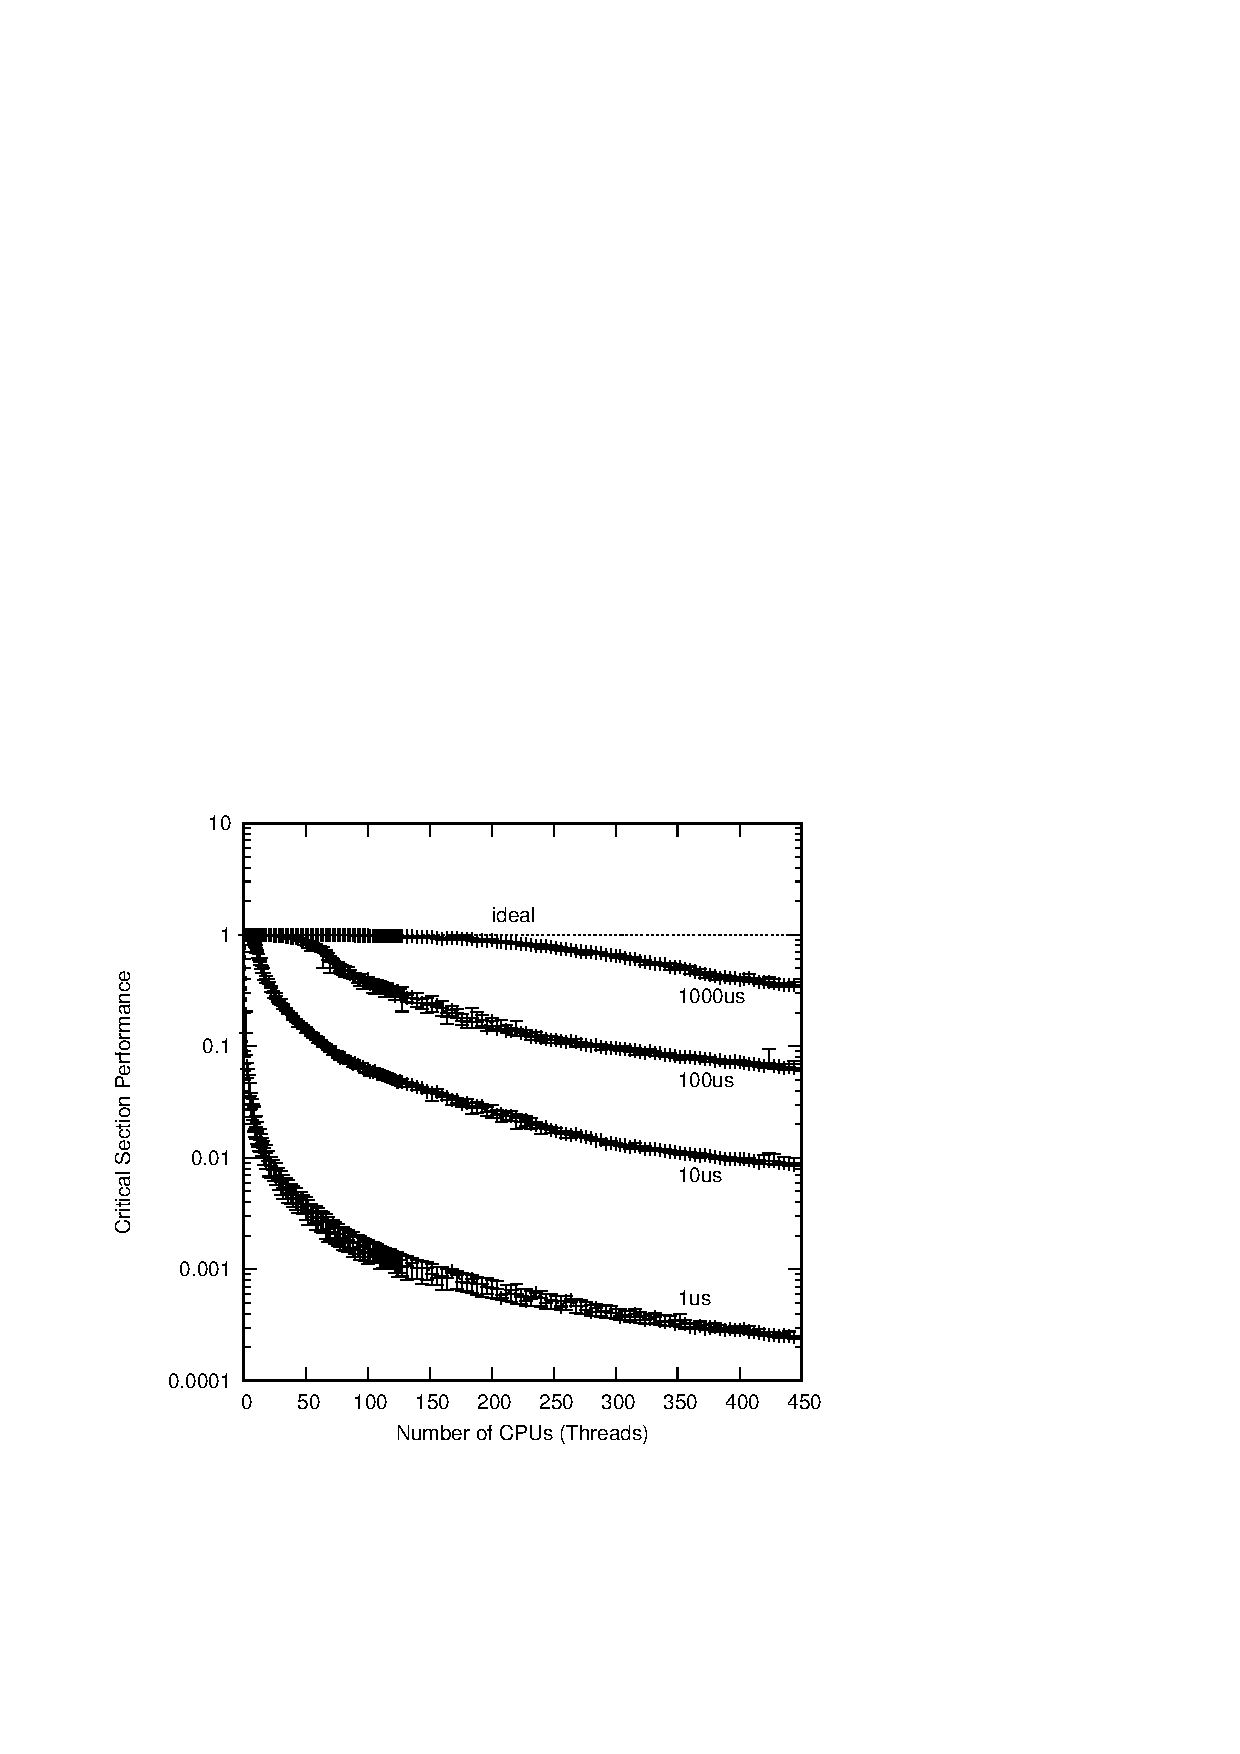
\includegraphics{CodeSamples/toolsoftrade/rwlockscale}}
\caption{Reader-Writer Lock Scalability vs. Microseconds in Critical Section on 8-Socket System With Intel Xeon Platinum 8176 CPUs @ 2.10GHz}
\label{fig:toolsoftrade:Reader-Writer Lock Scalability vs. Microseconds in Critical Section}
\end{figure}

Figure~\ref{fig:toolsoftrade:Reader-Writer Lock Scalability vs. Microseconds in Critical Section}
shows the results of running this test on a 224-core Xeon system
with two hardware threads per core for a total of 448 software-visible
CPUs.
The \co{thinktime} parameter was zero for all these tests, and the
\co{holdtime} parameter set to values ranging from one microsecond (``1us''
on the graph) to 10,000\,microseconds (``10000us'' on the graph).
The actual value plotted is:
\begin{equation}
	\frac{L_N}{N L_1}
\end{equation}
where $N$ is the number of threads,
$L_N$ is the number of lock acquisitions by $N$ threads, and
$L_1$ is the number of lock acquisitions by a single thread.
Given ideal hardware and software scalability, this value will always
be 1.0.

As can be seen in the figure, reader-writer locking scalability is
decidedly non-ideal, especially for smaller sizes of critical
sections.
To see why read-acquisition can be so slow, consider
that all the acquiring threads must update the \co{pthread_rwlock_t}
data structure.
Therefore, if all 448 executing threads attempt to
read-acquire the reader-writer lock concurrently, they must update
this underlying \co{pthread_rwlock_t} one at a time.
One lucky thread might do so almost immediately, but the least-lucky
thread must wait for all the other 447 threads to do their updates.
This situation will only get worse as you add CPUs.
Note also the logscale y-axis.
Even though the 10,000\,microsecond trace appears quite ideal, it has
in fact degraded by about 10\,\% from ideal.

\QuickQuizSeries{%
\QuickQuizB{
	Isn't comparing against single-CPU throughput a bit harsh?
}\QuickQuizAnswerB{
	Not at all.
	In fact, this comparison was, if anything, overly lenient.
	A more balanced comparison would be against single-CPU
	throughput with the locking primitives commented out.
}\QuickQuizEndB
%
\QuickQuizM{
	But one microsecond is not a particularly small size for
	a critical section.
	What do I do if I need a much smaller critical section, for
	example, one containing only a few instructions?
}\QuickQuizAnswerM{
	If the data being read \emph{never} changes, then you do not
	need to hold any locks while accessing it.
	If the data changes sufficiently infrequently, you might be
	able to checkpoint execution, terminate all threads, change
	the data, then restart at the checkpoint.

	Another approach is to keep a single exclusive lock per
	thread, so that a thread read-acquires the larger aggregate
	reader-writer lock by acquiring its own lock, and write-acquires
	by acquiring all the per-thread locks~\cite{WilsonCHsieh92a}.
	This can work quite well for readers, but causes writers
	to incur increasingly large overheads as the number of threads
	increases.

	Some other ways of efficiently handling very small critical
	sections are described in Chapter~\ref{chp:Deferred Processing}.
}\QuickQuizEndM
%
\QuickQuizM{
	The system used is a few years old, and new hardware should
	be faster.
	So why should anyone worry about reader-writer locks being slow?
}\QuickQuizAnswerE{
	In general, newer hardware is improving.
	However, it will need to improve several orders of magnitude
	to permit reader-writer lock to achieve ideal performance on
	448 CPUs.
	Worse yet, the greater the number of CPUs, the larger the
	required performance improvement.
	The performance problems of reader-writer locking are therefore
	very likely to be with us for quite some time to come.
}\QuickQuizEndE
}

Despite these limitations, reader-writer locking is quite useful in many
cases, for example when the readers must do high-latency file or network I/O.
There are alternatives, some of which will be presented in
Chapters~\ref{chp:Counting} and \ref{chp:Deferred Processing}.

\subsection{Atomic Operations (\GCC\ Classic)}
\label{sec:toolsoftrade:Atomic Operations (gcc Classic)}

Figure~\ref{fig:toolsoftrade:Reader-Writer Lock Scalability vs. Microseconds in Critical Section}
shows that the overhead of reader-writer locking is most severe for the
smallest critical sections, so it would be nice to have some other way
of protecting tiny critical sections.
One such way uses atomic operations.
\begin{fcvref}[ln:toolsoftrade:rwlockscale:reader:reader]
We have seen an atomic operation already, namely the
\apig{__sync_fetch_and_add()} primitive on \clnref{atmc_inc} of
Listing~\ref{lst:toolsoftrade:Measuring Reader-Writer Lock Scalability}.
This primitive atomically adds the value of its second argument to
the value referenced by its first argument, returning the old value
(which was ignored in this case).
If a pair of threads concurrently execute \co{__sync_fetch_and_add()} on
the same variable, the resulting value of the variable will include
the result of both additions.
\end{fcvref}

The \GNUC\ compiler offers a number of additional atomic operations,
including \apig{__sync_fetch_and_sub()},
\apig{__sync_fetch_and_or()},
\apig{__sync_fetch_and_and()},
\apig{__sync_fetch_and_xor()}, and
\apig{__sync_fetch_and_nand()}, all of which return the old value.
If you instead need the new value, you can instead use the
\apig{__sync_add_and_fetch()},
\apig{__sync_sub_and_fetch()},
\apig{__sync_or_and_fetch()},
\apig{__sync_and_and_fetch()},
\apig{__sync_xor_and_fetch()}, and
\apig{__sync_nand_and_fetch()} primitives.

\QuickQuiz{
	Is it really necessary to have both sets of primitives?
}\QuickQuizAnswer{
	Strictly speaking, no.
	One could implement any member of the second set using the
	corresponding member of the first set.
	For example, one could implement \apig{__sync_nand_and_fetch()}
	in terms of \apig{__sync_fetch_and_nand()} as follows:

\begin{VerbatimU}
tmp = v;
ret = __sync_fetch_and_nand(p, tmp);
ret = ~ret & tmp;
\end{VerbatimU}

	It is similarly possible to implement \apig{__sync_fetch_and_add()},
	\apig{__sync_fetch_and_sub()}, and \apig{__sync_fetch_and_xor()}
	in terms of their post-value counterparts.

	However, the alternative forms can be quite convenient, both
	for the programmer and for the compiler/library implementor.
}\QuickQuizEnd

The classic compare-and-swap operation is provided by a pair of
primitives, \apig{__sync_bool_compare_and_swap()} and
\apig{__sync_val_compare_and_swap()}.
Both of these primitive atomically update a location to a new value,
but only if its prior value was equal to the specified old value.
The first variant returns 1 if the operation succeeded and 0 if it
failed, for example, if the prior value was not equal to the specified
old value.
The second variant returns the prior value of the location, which, if
equal to the specified old value, indicates that the operation succeeded.
Either of the compare-and-swap operation is ``universal'' in the sense
that any atomic operation on a single location can be implemented in
terms of compare-and-swap, though the earlier operations are often
more efficient where they apply.
The compare-and-swap operation is also capable of serving as the basis
for a wider set of atomic operations, though the more elaborate of
these often suffer from complexity, scalability, and performance
problems~\cite{MauriceHerlihy90a}.

\QuickQuiz{
	Given that these atomic operations will often be able to
	generate single atomic instructions that are directly
	supported by the underlying instruction set, shouldn't
	they be the fastest possible way to get things done?
}\QuickQuizAnswer{
	Unfortunately, no.
	See Chapter~\ref{chp:Counting} for some stark counterexamples.
}\QuickQuizEnd

The \apig{__sync_synchronize()} primitive issues a ``memory barrier'',
which constrains both the compiler's and the CPU's ability to reorder
operations, as discussed in
Chapter~\ref{chp:Advanced Synchronization: Memory Ordering}.
In some cases, it is sufficient to constrain the compiler's ability
to reorder operations, while allowing the CPU free rein, in which
case the \apik{barrier()} primitive may be used.
\begin{fcvref}[ln:toolsoftrade:lock:reader_writer:reader]
In some cases, it is only necessary to ensure that the compiler
avoids optimizing away a given memory read, in which case the
\apik{READ_ONCE()} primitive may be used, as it was on \clnref{read_x} of
Listing~\ref{lst:toolsoftrade:Demonstration of Exclusive Locks}.
\end{fcvref}
Similarly, the \apik{WRITE_ONCE()} primitive may be used to prevent the
compiler from optimizing away a given memory write.
These last three primitives are not provided directly by \GCC,
but may be implemented straightforwardly as shown in
Listing~\ref{lst:toolsoftrade:Compiler Barrier Primitive (for GCC)},
and all three are discussed at length in
Section~\ref{sec:toolsoftrade:Accessing Shared Variables}.
Alternatively, \apialtk{READ_ONCE(x)}{READ_ONCE()} has much in common with
the \GCC\  intrinsic
\apialtg{__atomic_load_n(&x, __ATOMIC_RELAXED)}{__atomic_load_n()}
and \apik{WRITE_ONCE()} has much in common with the \GCC\ 
intrinsic \apialtg{__atomic_store_n(&x, v, __ATOMIC_RELAXED)}{__atomic_store_n()}.

\begin{listing}[tb]
\input{CodeSamples/api-pthreads/api-pthreads@compiler_barrier.fcv}
\caption{Compiler Barrier Primitive (for \GCC)}
\label{lst:toolsoftrade:Compiler Barrier Primitive (for GCC)}
\end{listing}

\QuickQuiz{
	What happened to \apikh{ACCESS_ONCE()}?
}\QuickQuizAnswer{
	As of early 2018, the Linux kernel's \apikh{ACCESS_ONCE()} is being
	replaced by \apik{READ_ONCE()} and \apik{WRITE_ONCE()} for reads and
	writes, respectively~\cite{JonCorbet2012ACCESS:ONCE,
	JonathanCorbet2014ACCESS:ONCEcompilerBugs,
	MarkRutland2017ACCESS:ONCE:remove}.
	\apikh{ACCESS_ONCE()} was introduced as a helper in RCU code, but was
	promoted to core API soon afterward~\cite{
	PaulEMcKenney2007ACCESS:ONCE:rcu,
	LinusTorvalds2008ACCESS:ONCE:move}.
	Linux kernel's \apik{READ_ONCE()} and \apik{WRITE_ONCE()} have
	evolved into complex forms that look quite different than
	the original \apikh{ACCESS_ONCE()} implementation due to the
	need to support access-once semantics for large structures,
	but with the possibility of load/store tearing if the structure
	cannot be loaded and stored with a single machine instruction.
}\QuickQuizEnd

\subsection{Atomic Operations (C11)}
\label{sec:toolsoftrade:Atomic Operations (C11)}

The C11 standard added atomic operations,
including loads (\apic{atomic_load()}),
stores (\apic{atomic_store()}),
memory barriers (\apic{atomic_thread_fence()} and
\apic{atomic_signal_fence()}), and read-modify-write atomics.
The read-modify-write atomics include
\apic{atomic_fetch_add()},
\apic{atomic_fetch_sub()},
\apic{atomic_fetch_and()},
\apic{atomic_fetch_xor()},
\apic{atomic_exchange()},
\apic{atomic_compare_exchange_strong()},
and
\apic{atomic_compare_exchange_weak()}.
These operate in a manner similar to those described in
Section~\ref{sec:toolsoftrade:Atomic Operations (gcc Classic)},
but with the addition of memory-order arguments to \co{_explicit}
variants of all of the operations.
Without memory-order arguments, all the atomic operations are
fully ordered, and the arguments permit weaker orderings.
For example, ``\apialtc{atomic_load_explicit(&a, memory_order_relaxed)}
{atomic_load_explicit()}''
is vaguely similar to the Linux kernel's ``\apik{READ_ONCE()}''.\footnote{
	Memory ordering is described in more detail in
	Chapter~\ref{chp:Advanced Synchronization: Memory Ordering} and
	Appendix~\ref{chp:app:whymb:Why Memory Barriers?}.}

\subsection{Atomic Operations (Modern \GCC)}
\label{sec:toolsoftrade:Atomic Operations (Modern gcc)}

One restriction of the C11 atomics is that they apply only to special
atomic types, which can be problematic.
The \GNUC\ compiler therefore provides atomic intrinsics, including
\apig{__atomic_load()},
\apig{__atomic_load_n()},
\apig{__atomic_store()},
\apig{__atomic_store_n()},
\apig{__atomic_thread_fence()}, etc.
These intrinsics offer the same semantics as their C11 counterparts,
but may be used on plain non-atomic objects.
Some of these intrinsics may be passed a memory-order argument from
this list:
\apig{__ATOMIC_RELAXED},
\apig{__ATOMIC_CONSUME},
\apig{__ATOMIC_ACQUIRE},
\apig{__ATOMIC_RELEASE},
\apig{__ATOMIC_ACQ_REL}, and
\apig{__ATOMIC_SEQ_CST}.

\subsection{Per-Thread Variables}
\label{sec:toolsoftrade:Per-Thread Variables}

Per-thread variables, also called thread-specific data, thread-local
storage, and other less-polite names, are used extremely
heavily in concurrent code, as will be explored in
Chapters~\ref{chp:Counting} and~\ref{chp:Data Ownership}.
POSIX supplies the \apipx{pthread_key_create()} function to create a
per-thread variable (and return the corresponding key),
\apipx{pthread_key_delete()} to delete the per-thread variable corresponding
to key,
\apipx{pthread_setspecific()} to set the value of the current thread's
variable corresponding to the specified key,
and \apipx{pthread_getspecific()} to return that value.

A number of compilers (including \GCC) provide a \apig{__thread} specifier
that may be used in a variable definition to designate that variable
as being per-thread.
The name of the variable may then be used normally to access the
value of the current thread's instance of that variable.
Of course, \apig{__thread} is much easier to use than the POSIX
thead-specific data, and so \co{__thread} is usually preferred for
code that is to be built only with \GCC\ or other compilers supporting
\co{__thread}.

Fortunately, the C11 standard introduced a \apic{_Thread_local} keyword
that can be used in place of \apig{__thread}.
In the fullness of time, this new keyword should combine the ease of use
of \co{__thread} with the portability of POSIX thread-specific data.

\section{Alternatives to POSIX Operations}
\label{sec:toolsoftrade:Alternatives to POSIX Operations}
%
\epigraph{The strategic marketing paradigm of Open Source is a massively
	  parallel drunkard's walk filtered by a Darwinistic process.}
	 {\emph{Bruce Perens}}

Unfortunately, threading operations, locking primitives, and atomic
operations were in reasonably wide use long before the various standards
committees got around to them.
As a result, there is considerable variation in how these operations
are supported.
It is still quite common to find these operations implemented in
assembly language, either for historical reasons or to obtain better
performance in specialized circumstances.
For example, \GCC's \co{__sync_} family of primitives all provide full
memory-ordering semantics, which in the past motivated many developers
to create their own implementations for situations where the full memory
ordering semantics are not required.
The following sections show some alternatives from the Linux kernel
and some historical primitives used by this book's sample code.

\subsection{Organization and Initialization}
\label{sec:toolsoftrade:Organization and Initialization}

Although many environments do not require any special initialization
code, the code samples in this book start with a call to \apipf{smp_init()},
which initializes a mapping from \apipx{pthread_t} to consecutive integers.
The userspace RCU library\footnote{
	See \cref{sec:defer:Read-Copy Update (RCU)} for more information
	on RCU.}
similarly requires a call to \apiur{rcu_init()}.
Although these calls can be hidden in environments (such as that of
\GCC) that support constructors,
most of the RCU flavors supported by the userspace RCU library
also require each thread invoke \apiur{rcu_register_thread()} upon thread
creation and \apiur{rcu_unregister_thread()} before thread exit.

In the case of the Linux kernel, it is a philosophical question as to
whether the kernel does not require calls to special initialization
code or whether the kernel's boot-time code is in fact the required
initialization code.

\subsection{Thread Creation, Destruction, and Control}
\label{sec:toolsoftrade:Thread Creation, Destruction, and Control}

The Linux kernel uses
\apik{struct task_struct} pointers to track kthreads,
\apik{kthread_create()} to create them,
\apik{kthread_should_stop()} to externally suggest that they stop
(which has no POSIX equivalent),
\apik{kthread_stop()} to wait for them to stop, and
\apik{schedule_timeout_interruptible()} for a timed wait.
There are quite a few additional kthread-management APIs, but this
provides a good start, as well as good search terms.

The CodeSamples API focuses on ``threads'', which are a locus of
control.\footnote{
	There are many other names for similar software constructs, including
	``process'', ``task'', ``fiber'', ``event'', ``execution agent'',
	and so on.
	Similar design principles apply to all of them.}
Each such thread has an identifier of type \apipf{thread_id_t},
and no two threads running at a given time will have the same
identifier.
Threads share everything except for per-thread local state,\footnote{
	How is that for a circular definition?}
which includes program counter and stack.

The thread API is shown in
Listing~\ref{lst:toolsoftrade:Thread API}, and members are described in the
following sections.

\begin{listing}[tbp]
\begin{VerbatimL}[numbers=none,xleftmargin=2pt]
int smp_thread_id(void)
thread_id_t create_thread(void *(*func)(void *), void *arg)
for_each_thread(t)
for_each_running_thread(t)
void *wait_thread(thread_id_t tid)
void wait_all_threads(void)
\end{VerbatimL}
\caption{Thread API}
\label{lst:toolsoftrade:Thread API}
\end{listing}

\subsubsection{\tco{create_thread()}}

The \apipf{create_thread()} primitive creates a new thread,
starting the new thread's execution
at the function \co{func} specified by \apipf{create_thread()}'s
first argument, and passing it the argument specified by
\apipf{create_thread()}'s second argument.
This newly created thread will terminate when it returns from the
starting function specified by \co{func}.
The \apipf{create_thread()} primitive returns the \apipf{thread_id_t}
corresponding to the newly created child thread.

This primitive will abort the program if more than \apipf{NR_THREADS}
threads are created, counting the one implicitly created by running
the program.
\apipf{NR_THREADS} is a compile-time constant that may be modified,
though some systems may have an upper bound for the allowable number
of threads.

\subsubsection{\tco{smp_thread_id()}}

Because the \apipf{thread_id_t} returned from \apipf{create_thread()} is
system-dependent, the \apipf{smp_thread_id()} primitive returns a thread
index corresponding to the thread making the request.
This index is guaranteed to be less than the maximum number of threads
that have been in existence since the program started,
and is therefore useful for bitmasks, array indices, and
the like.

\subsubsection{\tco{for_each_thread()}}

The \apipf{for_each_thread()} macro loops through all threads that exist,
including all threads that \emph{would} exist if created.
This macro is useful for handling per-thread variables as will be
seen in Section~\ref{sec:toolsoftrade:Per-Thread Variables}.

\subsubsection{\tco{for_each_running_thread()}}

The \apipf{for_each_running_thread()}
macro loops through only those threads that currently exist.
It is the caller's responsibility to synchronize with thread
creation and deletion if required.

\subsubsection{\tco{wait_thread()}}

The \apipf{wait_thread()} primitive waits for completion of the thread
specified by the \co{thread_id_t} passed to it.
This in no way interferes with the execution of the specified thread;
instead, it merely waits for it.
Note that \apipf{wait_thread()} returns the value that was returned by
the corresponding thread.

\subsubsection{\tco{wait_all_threads()}}

The \apipf{wait_all_threads()}
primitive waits for completion of all currently running threads.
It is the caller's responsibility to synchronize with thread creation
and deletion if required.
However, this primitive is normally used to clean up at the end of
a run, so such synchronization is normally not needed.

\subsubsection{Example Usage}

Listing~\ref{lst:toolsoftrade:Example Child Thread} (\path{threadcreate.c})
shows an example hello-world-like child thread.
As noted earlier, each thread is allocated its own stack, so
each thread has its own private \co{arg} argument and \co{myarg} variable.
Each child simply prints its argument and its \apipf{smp_thread_id()}
before exiting.
Note that the \co{return} statement on
line~\ref{ln:intro:threadcreate:thread_test:return} terminates the thread,
returning a \co{NULL} to whoever invokes \apipf{wait_thread()} on this
thread.

\begin{listing}[tbp]
\input{CodeSamples/intro/threadcreate@thread_test.fcv}
\caption{Example Child Thread}
\label{lst:toolsoftrade:Example Child Thread}
\end{listing}

\begin{fcvref}[ln:intro:threadcreate:main]
The parent program is shown in
Listing~\ref{lst:toolsoftrade:Example Parent Thread}.
It invokes \co{smp_init()} to initialize the threading system on
line~\lnref{smp_init},
parses arguments on \clnrefrange{parse:b}{parse:e},
and announces its presence on line~\lnref{announce}.
It creates the specified number of child threads on
\clnrefrange{create:b}{create:e},
and waits for them to complete on line~\lnref{wait}.
Note that \apipf{wait_all_threads()} discards the threads return values,
as in this case they are all \co{NULL}, which is not very interesting.
\end{fcvref}

\begin{listing}[tbp]
\input{CodeSamples/intro/threadcreate@main.fcv}
\caption{Example Parent Thread}
\label{lst:toolsoftrade:Example Parent Thread}
\end{listing}

\QuickQuiz{
	What happened to the Linux-kernel equivalents to \apipx{fork()}
	and \apipx{wait()}?
}\QuickQuizAnswer{
	They don't really exist.
	All tasks executing within the Linux kernel share memory,
	at least unless you want to do a huge amount of memory-mapping
	work by hand.
}\QuickQuizEnd

\subsection{Locking}
\label{sec:toolsoftrade:Locking}

A good starting subset of the Linux kernel's locking API is shown in
Listing~\ref{lst:toolsoftrade:Locking API},
each API element being described in the following sections.
This book's CodeSamples locking API closely follows that of the Linux kernel.

\begin{listing}[tbp]
\begin{VerbatimL}[numbers=none]
void spin_lock_init(spinlock_t *sp);
void spin_lock(spinlock_t *sp);
int spin_trylock(spinlock_t *sp);
void spin_unlock(spinlock_t *sp);
\end{VerbatimL}
\caption{Locking API}
\label{lst:toolsoftrade:Locking API}
\end{listing}

\subsubsection{\tco{spin_lock_init()}}

The \apik{spin_lock_init()} primitive initializes the specified
\apik{spinlock_t} variable, and must be invoked before
this variable is passed to any other spinlock primitive.

\subsubsection{\tco{spin_lock()}}

The \apik{spin_lock()} primitive acquires the specified spinlock,
if necessary, waiting until the spinlock becomes available.
In some environments, such as pthreads, this waiting will involve
blocking, while in others, such as the Linux kernel, it might involve
a CPU-bound spin loop.

The key point is that only one thread may hold a spinlock at any
given time.

\subsubsection{\tco{spin_trylock()}}

The \apik{spin_trylock()} primitive acquires the specified spinlock,
but only if it is immediately available.
It returns \co{true} if it was able to acquire the spinlock and
\co{false} otherwise.

\subsubsection{\tco{spin_unlock()}}

The \apik{spin_unlock()} primitive releases the specified spinlock,
allowing other threads to acquire it.

% \emph{@@@ likely need to add reader-writer locking.}

\subsubsection{Example Usage}

A spinlock named \co{mutex} may be used to protect a variable
\co{counter} as follows:

\begin{VerbatimU}
spin_lock(&mutex);
counter++;
spin_unlock(&mutex);
\end{VerbatimU}

\QuickQuiz{
	What problems could occur if the variable {\tt counter} were
	incremented without the protection of {\tt mutex}?
}\QuickQuizAnswer{
	On CPUs with load-store architectures, incrementing {\tt counter}
	might compile into something like the following:

\begin{VerbatimU}
LOAD counter,r0
INC r0
STORE r0,counter
\end{VerbatimU}

	On such machines, two threads might simultaneously load the
	value of {\tt counter}, each increment it, and each store the
	result.
	The new value of {\tt counter} will then only be one greater
	than before, despite two threads each incrementing it.
}\QuickQuizEnd

However, the \apik{spin_lock()} and \apik{spin_unlock()} primitives
do have performance consequences, as will be seen in
Chapter~\ref{chp:Data Structures}.

\subsection{Accessing Shared Variables}
\label{sec:toolsoftrade:Accessing Shared Variables}

It was not until 2011 that the C standard defined semantics for concurrent
read/write access to shared variables.
However, concurrent C code was being written at least a quarter century
earlier~\cite{Beck85,Inman85}.
This raises the question as to what today's greybeards did back
in long-past pre-C11 days.
A short answer to this question is ``they lived dangerously''.

\begin{listing}[tbp]
\begin{fcvlabel}[ln:toolsoftrade:Living Dangerously Early 1990s Style]
\begin{VerbatimL}[commandchars=\\\{\}]
ptr = global_ptr;\lnlbl{temp}
if (ptr != NULL && ptr < high_address)
	do_low(ptr);
\end{VerbatimL}
\end{fcvlabel}
\caption{Living Dangerously Early 1990s Style}
\label{lst:toolsoftrade:Living Dangerously Early 1990s Style}
\end{listing}

\begin{listing}[tbp]
\begin{fcvlabel}[ln:toolsoftrade:C Compilers Can Invent Loads]
\begin{VerbatimL}[commandchars=\\\{\}]
if (global_ptr != NULL &&\lnlbl{if:a}
    global_ptr < high_address)\lnlbl{if:b}
	do_low(global_ptr);\lnlbl{do_low}
\end{VerbatimL}
\end{fcvlabel}
\caption{C Compilers Can Invent Loads}
\label{lst:toolsoftrade:C Compilers Can Invent Loads}
\end{listing}

At least they would have been living dangerously had they been using
2018 compilers.
In (say) the early 1990s, compilers did fewer optimizations, in part
because there were fewer compiler writers and in part due to the
relatively small memories of that era.
Nevertheless, problems did arise, as shown in
Listing~\ref{lst:toolsoftrade:Living Dangerously Early 1990s Style},
which the compiler is within its rights to transform into
Listing~\ref{lst:toolsoftrade:C Compilers Can Invent Loads}.
As you can, the temporary on
line~\ref{ln:toolsoftrade:Living Dangerously Early 1990s Style:temp} of
Listing~\ref{lst:toolsoftrade:Living Dangerously Early 1990s Style}
has been optimized away, so that \co{global_ptr} will be loaded
up to three times.

\QuickQuiz{
	What is wrong with loading
	Listing~\ref{lst:toolsoftrade:Living Dangerously Early 1990s Style}'s
	\co{global_ptr} up to three times?
}\QuickQuizAnswer{
	Suppose that \co{global_ptr} is initially non-\co{NULL},
	but that some other thread sets \co{global_ptr} to \co{NULL}.
	\begin{fcvref}[ln:toolsoftrade:C Compilers Can Invent Loads]
	Suppose further that line~\lnref{if:a} of the transformed code
	(Listing~\ref{lst:toolsoftrade:C Compilers Can Invent Loads})
	executes just before \co{global_ptr} is set to \co{NULL} and
	line~\lnref{if:b} just after.
	Then line~\lnref{if:a} will conclude that
        \co{global_ptr} is non-\co{NULL},
	line~\lnref{if:b} will conclude that it is less than
        \co{high_address},
	so that line~\lnref{do_low} passes \co{do_low()} a \co{NULL} pointer,
	which \co{do_low()} just might not be prepared to deal with.
	\end{fcvref}

	Your editor made exactly this mistake in the DYNIX/ptx
	kernel's memory allocator in the early 1990s.
	Tracking down the bug consumed a holiday weekend not just
	for your editor, but also for several of his colleagues.
	In short, this is not a new problem, nor is it likely to
	go away on its own.
}\QuickQuizEnd

Section~\ref{sec:toolsoftrade:Shared-Variable Shenanigans}
describes additional problems caused by plain accesses,
Sections~\ref{sec:toolsoftrade:A Volatile Solution}
and~\ref{sec:toolsoftrade:Assembling the Rest of a Solution}
describe some pre-C11 solutions.
Of course, where practical, the primitives described in
Section~\ref{sec:toolsoftrade:Atomic Operations (gcc Classic)}
or (especially)
Section~\ref{sec:toolsoftrade:Atomic Operations (C11)}
should instead be used to avoid data races, that is, to ensure
that if there are multiple concurrent accesses to a given
variable, all of those accesses are loads.

\subsubsection{Shared-Variable Shenanigans}
\label{sec:toolsoftrade:Shared-Variable Shenanigans}
\OriginallyPublished{Section}{sec:toolsoftrade:Shared-Variable Shenanigans}{Shared-Variable Shenanigans}{Linux Weekly News}{JadeAlglave2019WhoAfraidCompiler}
%
Given code that does plain loads and stores,\footnote{
	That is, normal loads and stores instead of C11 atomics, inline
	assembly, or volatile accesses.}
the compiler is within
its rights to assume that the affected variables are neither accessed
nor modified by any other thread.
This assumption allows the compiler to carry out a large number of
transformations, including load tearing, store tearing,
load fusing, store fusing, code reordering, invented loads,
invented stores, store-to-load transformations, and dead-code elimination,
all of which work just fine in single-threaded code.
But concurrent code can be broken by each of these transformations,
or shared-variable shenanigans, as described below.

{\bf Load tearing} occurs when the compiler uses multiple load
instructions for a single access.
For example, the compiler could in theory compile the load from
\co{global_ptr} (see
line~\ref{ln:toolsoftrade:Living Dangerously Early 1990s Style:temp} of
Listing~\ref{lst:toolsoftrade:Living Dangerously Early 1990s Style})
as a series of one-byte loads.
If some other thread was concurrently setting \co{global_ptr} to
\co{NULL}, the result might have all but one byte of the pointer
set to zero, thus forming a ``wild pointer''.
Stores using such a wild pointer could corrupt arbitrary
regions of memory, resulting in rare and difficult-to-debug crashes.

Worse yet, on (say) an 8-bit system with 16-bit pointers, the compiler
might have no choice but to use a pair of 8-bit instructions to access
a given pointer.
Because the C standard must support all manner of systems, the standard
cannot rule out load tearing in the general case.

{\bf Store tearing} occurs when the compiler uses multiple store
instructions for a single access.
For example, one thread might store \co{0x12345678} to a four-byte integer
variable at the same time another thread stored \co{0xabcdef00}.
If the compiler used 16-bit stores for either access, the result
might well be \co{0x1234ef00}, which could come as quite a surprise to
code loading from this integer.
Nor is this a strictly theoretical issue.
For example, there are CPUs that feature small immediate instruction
fields, and on such CPUs, the compiler might split a 64-bit store into
two 32-bit stores in order to reduce the overhead of explicitly forming
the 64-bit constant in a register, even on a 64-bit CPU.
There are historical reports of this actually happening in
the wild (e.g.~\cite{KonstantinKhlebnikov2013gccstoretearing}),
but there is also a recent
report~\cite{WillDeacon2019StoreTearingReport}.\footnote{
	Note that this tearing can happen even on properly aligned
        and machine-word-sized accesses, and in this particular case,
	even for volatile stores.
	Some might argue that this behavior constitutes a bug in the
	compiler, but either way it illustrates the perceived value of
	store tearing from a compiler-writer viewpoint.
}

Of course, the compiler simply has no choice but to tear some stores
in the general case, given
the possibility of code using 64-bit integers running on a 32-bit system.
But for properly aligned machine-sized stores, \apik{WRITE_ONCE()} will
prevent store tearing.

\begin{listing}[tbp]
\begin{fcvlabel}[ln:toolsoftrade:Preventing Load Fusing]
\begin{VerbatimL}[commandchars=\\\{\}]
while (!need_to_stop)
	do_something_quickly();
\end{VerbatimL}
\end{fcvlabel}
\caption{Inviting Load Fusing}
\label{lst:toolsoftrade:Inviting Load Fusing}
\end{listing}

\begin{listing}[tbp]
\begin{fcvlabel}[ln:toolsoftrade:C Compilers Can Fuse Loads]
\begin{VerbatimL}[commandchars=\\\[\]]
if (!need_to_stop)
	for (;;) {\lnlbl[loop:b]
		do_something_quickly();
		do_something_quickly();
		do_something_quickly();
		do_something_quickly();
		do_something_quickly();
		do_something_quickly();
		do_something_quickly();
		do_something_quickly();
		do_something_quickly();
		do_something_quickly();
		do_something_quickly();
		do_something_quickly();
		do_something_quickly();
		do_something_quickly();
		do_something_quickly();
		do_something_quickly();
	}\lnlbl[loop:e]
\end{VerbatimL}
\end{fcvlabel}
\caption{C Compilers Can Fuse Loads}
\label{lst:toolsoftrade:C Compilers Can Fuse Loads}
\end{listing}

{\bf Load fusing} occurs when the compiler uses the result of a
prior load from a given variable instead of repeating the load.
Not only is this sort of optimization just fine in single-threaded
code, it is often just fine in multithreaded code.
Unfortunately, the word ``often'' hides some truly annoying exceptions.

For example, suppose that a real-time system needs to invoke a
function named \co{do_something_quickly()} repeatedly until the
variable \co{need_to_stop} was set, and that the compiler can see
that \co{do_something_quickly()} does not store to \co{need_to_stop}.
One (unsafe) way to code this is shown in
Listing~\ref{lst:toolsoftrade:Inviting Load Fusing}.
The compiler might reasonably unroll this loop sixteen times in order
to reduce the per-invocation of the backwards branch at the end of the
loop.
Worse yet, because the compiler knows that \co{do_something_quickly()}
does not store to \co{need_to_stop}, the compiler could quite reasonably
decide to check this variable only once, resulting in the code shown in
Listing~\ref{lst:toolsoftrade:C Compilers Can Fuse Loads}.
\begin{fcvref}[ln:toolsoftrade:C Compilers Can Fuse Loads]
Once entered, the loop on
\clnrefrange{loop:b}{loop:e} will never exit, regardless of how
many times some other thread stores a non-zero value to \co{need_to_stop}.
\end{fcvref}
The result will at best be consternation, and might well also
include severe physical damage.

\begin{listing}[tbp]
\begin{fcvlabel}[ln:toolsoftrade:C Compilers Can Fuse Non-Adjacent Loads]
\begin{VerbatimL}[commandchars=\\\[\]]
int *gp; \lnlbl[gp]

void t0(void)
{
	WRITE_ONCE(gp, &myvar); \lnlbl[wgp]
}

void t1(void)
{
	p1 = gp; \lnlbl[p1]
	do_something(p1);
	p2 = READ_ONCE(gp); \lnlbl[p2]
	if (p2) { \lnlbl[if]
		do_something_else();
		p3 = *gp; \lnlbl[p3]
	}
}
\end{VerbatimL}
\end{fcvlabel}
\caption{C Compilers Can Fuse Non-Adjacent Loads}
\label{lst:toolsoftrade:C Compilers Can Fuse Non-Adjacent Loads}
\end{listing}

\begin{fcvref}[ln:toolsoftrade:C Compilers Can Fuse Non-Adjacent Loads]
The compiler can fuse loads across surprisingly large spans of code.
For example, in
Listing~\ref{lst:toolsoftrade:C Compilers Can Fuse Non-Adjacent Loads},
\co{t0()} and \co{t1()} run concurrently, and \co{do_something()} and
\co{do_something_else()} are inline functions.
Line~\lnref{gp} declares pointer \co{gp}, which C initializes to \co{NULL}
by default.
At some point, line~\lnref{wgp} of \co{t0()} stores a non-\co{NULL}
pointer to \co{gp}.
Meanwhile, \co{t1()} loads from \co{gp} three times on
lines~\lnref{p1}, \lnref{p2}, and~\lnref{p3}.
Given that line~\lnref{if} finds that \co{gp} is non-\co{NULL}, one might
hope that the dereference on line~\lnref{p3} would be guaranteed never
to fault.
Unfortunately, the compiler is within its rights to fuse the read on
lines~\lnref{p1} and~\lnref{p3}, which means that if line~\lnref{p1}
loads \co{NULL} and line~\lnref{p2} loads \co{&myvar}, line~\lnref{p3}
could load \co{NULL}, resulting in a fault.\footnote{
	\ppl{Will}{Deacon} reports that this happened in the Linux kernel.}
Note that the intervening \apik{READ_ONCE()} does not prevent the other
two loads from being fused, despite the fact that all three are loading
from the same variable.
\end{fcvref}

\QuickQuiz{
	Why does it matter whether \co{do_something()} and
	\co{do_something_else()} in
	Listing~\ref{lst:toolsoftrade:C Compilers Can Fuse Non-Adjacent Loads}
	are inline functions?
}\QuickQuizAnswer{
	\begin{fcvref}[ln:toolsoftrade:C Compilers Can Fuse Non-Adjacent Loads]
	Because \co{gp} is not a static variable, if either
	\co{do_something()} or \co{do_something_else()} were separately
	compiled, the compiler would have to assume that either or both
	of these two functions might change the value of \co{gp}.
	This possibility would force the compiler to reload \co{gp}
	on line~\lnref{p3}, thus avoiding the \co{NULL}-pointer dereference.
	\end{fcvref}
}\QuickQuizEnd

{\bf Store fusing} can occur when the compiler notices a pair of successive
stores to a given variable with no intervening loads from that variable.
In this case, the compiler is within its rights to omit the first store.
This is never a problem in single-threaded code, and in fact it is
usually not a problem in correctly written concurrent code.
After all, if the two stores are executed in quick succession, there is
very little chance that some other thread could load the value from the
first store.

\begin{listing}[tbp]
\begin{fcvlabel}[ln:toolsoftrade:C Compilers Can Fuse Stores]
\begin{VerbatimL}[commandchars=\\\[\]]
void shut_it_down(void)
{
	status = SHUTTING_DOWN; /* BUGGY!!! */\lnlbl[store:a]
	start_shutdown();
	while (!other_task_ready) /* BUGGY!!! */\lnlbl[loop:b]
		continue;\lnlbl[loop:e]
	finish_shutdown();\lnlbl[finish]
	status = SHUT_DOWN; /* BUGGY!!! */\lnlbl[store:b]
	do_something_else();
}

void work_until_shut_down(void)
{
	while (status != SHUTTING_DOWN) /* BUGGY!!! */\lnlbl[until:loop:b]
		do_more_work();\lnlbl[until:loop:e]
	other_task_ready = 1; /* BUGGY!!! */\lnlbl[other:store]
}
\end{VerbatimL}
\end{fcvlabel}
\caption{C Compilers Can Fuse Stores}
\label{lst:toolsoftrade:C Compilers Can Fuse Stores}
\end{listing}

However, there are exceptions, for example as shown in
Listing~\ref{lst:toolsoftrade:C Compilers Can Fuse Stores}.
\begin{fcvref}[ln:toolsoftrade:C Compilers Can Fuse Stores]
The function \co{shut_it_down()} stores to the shared
variable \co{status} on lines~\lnref{store:a} and~\lnref{store:b},
and so assuming that neither
\co{start_shutdown()} nor \co{finish_shutdown()} access \co{status},
the compiler could reasonably remove the store to \co{status} on
line~\lnref{store:a}.
Unfortunately, this would mean that \co{work_until_shut_down()} would
never exit its loop spanning
lines~\lnref{until:loop:b} and~\lnref{until:loop:e}, and thus would never set
\co{other_task_ready}, which would in turn mean that \co{shut_it_down()}
would never exit its loop spanning
lines~\lnref{loop:b} and~\lnref{loop:e}, even if
the compiler chooses not to fuse the successive loads from
\co{other_task_ready} on line~\lnref{loop:b}.

And there are more problems with the code in
Listing~\ref{lst:toolsoftrade:C Compilers Can Fuse Stores},
including code reordering.

{\bf Code reordering} is a common compilation technique used to
combine common subexpressions, reduce register pressure, and
improve utilization of the many functional units available on
modern superscalar microprocessors.
It is also another reason why the code in
Listing~\ref{lst:toolsoftrade:C Compilers Can Fuse Stores}
is buggy.
For example, suppose that the \co{do_more_work()} function on
line~\lnref{until:loop:e}
does not access \co{other_task_ready}.
Then the compiler would be within its rights to move the assignment
to \co{other_task_ready} on
line~\lnref{other:store} to precede line~\lnref{until:loop:b}, which might
be a great disappointment for anyone hoping that the last call to
\co{do_more_work()} on line~\lnref{until:loop:e} happens before the call to
\co{finish_shutdown()} on line~\lnref{finish}.
\end{fcvref}

It might seem futile to prevent the compiler from changing the order of
accesses in cases where the underlying hardware is free to reorder them.
However, modern machines have \emph{exact exceptions} and
\emph{exact interrupts}, meaning that any interrupt or exception will
appear to have happened at a specific place in the instruction
stream.
This means that the handler will see the effect of all prior
instructions, but won't see the effect of any subsequent instructions.
\apik{READ_ONCE()} and \apik{WRITE_ONCE()} can therefore be used to
control communication between interrupted code and interrupt handlers,
independent of the ordering provided by the underlying hardware.\footnote{
	That said, the various standards committees would prefer that
	you use atomics or variables of type \apic{sig_atomic_t}, instead
	of \apik{READ_ONCE()} and \apik{WRITE_ONCE()}.}

{\bf Invented loads} were illustrated by the code in
Listings~\ref{lst:toolsoftrade:Living Dangerously Early 1990s Style}
and~\ref{lst:toolsoftrade:C Compilers Can Invent Loads},
in which the compiler optimized away a temporary variable,
thus loading from a shared variable more often than intended.

Invented loads can be a performance hazard.
These hazards can occur when a load of variable in a ``hot''
cacheline is hoisted out of an \co{if} statement.
These hoisting optimizations are not uncommon, and can cause significant
increases in cache misses, and thus significant degradation of
both performance and scalability.

\begin{fcvref}[ln:toolsoftrade:C Compilers Can Fuse Stores]
{\bf Invented stores} can occur in a number of situations.
For example, a compiler emitting code for \co{work_until_shut_down()} in
Listing~\ref{lst:toolsoftrade:C Compilers Can Fuse Stores}
might notice that \co{other_task_ready} is not accessed by
\co{do_more_work()}, and stored to on line~\lnref{other:store}.
If \co{do_more_work()} was a complex inline function, it might be
necessary to do a register spill, in which case one attractive
place to use for temporary storage is \co{other_task_ready}.
After all, there are no accesses to it, so what is the harm?

Of course, a non-zero store to this variable at just the wrong time
would result in the \co{while} loop on
line~\lnref{loop:b} terminating
prematurely, again allowing \co{finish_shutdown()} to run
concurrently with \co{do_more_work()}.
Given that the entire point of this \co{while} appears to be to
prevent such concurrency, this is not a good thing.
\end{fcvref}

\begin{listing}[tbp]
\begin{fcvlabel}[ln:toolsoftrade:Inviting an Invented Store]
\begin{VerbatimL}[commandchars=\\\{\}]
if (condition)
	a = 1;
else
	do_a_bunch_of_stuff();
\end{VerbatimL}
\end{fcvlabel}
\caption{Inviting an Invented Store}
\label{lst:toolsoftrade:Inviting an Invented Store}
\end{listing}

\begin{listing}[tbp]
\begin{fcvlabel}[ln:toolsoftrade:Compiler Invents an Invited Store]
\begin{VerbatimL}[commandchars=\\\[\]]
a = 1;\lnlbl[store:uncond]
if (!condition) {
	a = 0;\lnlbl[store:cond]
	do_a_bunch_of_stuff();
}
\end{VerbatimL}
\end{fcvlabel}
\caption{Compiler Invents an Invited Store}
\label{lst:toolsoftrade:Compiler Invents an Invited Store}
\end{listing}

Using a stored-to variable as a temporary might seem outlandish,
but it is permitted by the standard.
Nevertheless, readers might be justified in wanting a less
outlandish example, which is provided by
Listings~\ref{lst:toolsoftrade:Inviting an Invented Store}
and~\ref{lst:toolsoftrade:Compiler Invents an Invited Store}.

A compiler emitting code for
Listing~\ref{lst:toolsoftrade:Inviting an Invented Store}
might know that the value of \co{a} is initially zero,
which might be a strong temptation to optimize away one branch
by transforming this code to that in
Listing~\ref{lst:toolsoftrade:Compiler Invents an Invited Store}.
\begin{fcvref}[ln:toolsoftrade:Compiler Invents an Invited Store]
Here, line~\lnref{store:uncond} unconditionally stores \co{1} to \co{a}, then
resets the value back to zero on
line~\lnref{store:cond} if \co{condition} was not set.
This transforms the if-then-else into an if-then, saving one branch.
\end{fcvref}

\QuickQuiz{
	Ouch!
	So can't the compiler invent a store to a normal variable pretty
	much any time it likes?
}\QuickQuizAnswer{
	Thankfully, the answer is no.
	This is because the compiler is forbidden from introducing data races.
	The case of inventing a store just before a normal store is
	quite special:  It is not possible for some other entity,
	be it CPU, thread, signal handler, or interrupt handler, to be
	able to see the invented store unless the code already has
	a data race, even without the invented store.
	And if the code already has a data race, it already invokes
	the dreaded spectre of undefined behavior, which allows the
	compiler to generate pretty much whatever code it wants,
	regardless of the wishes of the developer.

	But if the original store is volatile, as in \apik{WRITE_ONCE()},
	for all the compiler knows, there might be a side effect
	associated with the store that could signal some other thread,
	allowing data-race-free access to the variable.
	By inventing the store, the compiler might be introducing a
	data race, which it is not permitted to do.

	In the case of \co{volatile} and atomic variables, the compiler
	is specifically forbidden from inventing writes.
}\QuickQuizEnd

Finally, pre-C11 compilers could invent writes to unrelated
variables that happened to be adjacent to written-to
variables~\cite[Section 4.2]{Boehm:2005:TCI:1064978.1065042}.
This variant of invented stores has been outlawed by the prohibition
against compiler optimizations that invent data races.

\begin{listing}[tbp]
\begin{fcvlabel}[ln:toolsoftrade:Inviting a Store-to-Load Conversion]
\begin{VerbatimL}[commandchars=\\\[\]]
r1 = p;\lnlbl[load:p]
if (unlikely(r1))\lnlbl[if]
	do_something_with(r1);\lnlbl[dsw]
barrier();\lnlbl[barrier]
p = NULL;\lnlbl[null]
\end{VerbatimL}
\end{fcvlabel}
\caption{Inviting a Store-to-Load Conversion}
\label{lst:toolsoftrade:Inviting a Store-to-Load Conversion}
\end{listing}

{\bf Store-to-load transformations} can occur when the compiler notices
that a plain store might not actually change the value in memory.
\begin{fcvref}[ln:toolsoftrade:Inviting a Store-to-Load Conversion]
For example, consider
Listing~\ref{lst:toolsoftrade:Inviting a Store-to-Load Conversion}.
Line~\lnref{load:p} fetches \co{p}, but the \qco{if} statement on
line~\lnref{if} also tells the compiler that the developer thinks that
\co{p} is usually zero.\footnote{
	The \apik{unlikely()} function provides this hint to the compiler,
	and different compilers provide different ways of implementing
	\co{unlikely()}.}
The \apik{barrier()} statment on line~\lnref{barrier} forces the compiler
to forget the value of \co{p}, but one could imagine a compiler
choosing to remember the hint---or getting an additional hint via
feedback-directed optimization.
Doing so would cause the compiler to realize that line~\lnref{null}
is often an expensive no-op.
\end{fcvref}

\begin{listing}[tbp]
\begin{fcvlabel}[ln:toolsoftrade:Compiler Converts a Store to a Load]
\begin{VerbatimL}[commandchars=\\\[\]]
r1 = p;\lnlbl[load:p]
if (unlikely(r1))\lnlbl[if]
	do_something_with(r1);\lnlbl[dsw]
barrier();\lnlbl[barrier]
if (p != NULL)\lnlbl[if1]
	p = NULL;\lnlbl[null]
\end{VerbatimL}
\end{fcvlabel}
\caption{Compiler Converts a Store to a Load}
\label{lst:toolsoftrade:Compiler Converts a Store to a Load}
\end{listing}

\begin{fcvref}[ln:toolsoftrade:Compiler Converts a Store to a Load]
Such a compiler might therefore guard the store of \co{NULL}
with a check, as shown on lines~\lnref{if1} and~\lnref{null} of
Listing~\ref{lst:toolsoftrade:Compiler Converts a Store to a Load}.
Although this transformation is often desirable, it could be problematic
if the actual store was required for ordering.
For example, a write memory barrier (Linux kernel \apik{smp_wmb()}) would
order the store, but not the load.
This situation might suggest use of \apik{smp_store_release()} over
\apik{smp_wmb()}.
\end{fcvref}

{\bf Dead-code elimination} can occur when the compiler notices that
the value from a load is never used, or when a variable is stored to,
but never loaded from.
This can of course eliminate an access to a shared variable, which
can in turn defeat a memory-ordering primitive, which could cause your
concurrent code to act in surprising ways.
Experience thus far indicates that relatively few such surprises will
be at all pleasant.
Elimination of store-only variables is especially dangerous in cases
where external code locates the variable via symbol tables: The
compiler is necessarily ignorant of such external-code accesses, and
might thus eliminate a variable that the external code relies upon.

Reliable concurrent code clearly needs a way to cause the compiler to
preserve the number, order, and type of important accesses to shared
memory, a topic taken up by
Sections~\ref{sec:toolsoftrade:A Volatile Solution}
and~\ref{sec:toolsoftrade:Assembling the Rest of a Solution},
which are up next.

\subsubsection{A Volatile Solution}
\label{sec:toolsoftrade:A Volatile Solution}

Although it is now much maligned, before the advent of C11 and
C++11~\cite{PeteBecker2011N3242}, the \apic{volatile} keyword was an
indispensible tool in the parallel programmer's toolbox.
This raises the question of exactly what \co{volatile} means,
a question that is not answered with excessive precision even
by more recent versions of this standard~\cite{RichardSmith2018N4762}.\footnote{
	JF Bastien thoroughly documented the history and use cases
	for the \co{volatile} keyword in
	C++~\cite{JFBastien2018DeprecatingVolatile}.}
This version guarantees that ``Accesses through \co{volatile}
\co{glvalues} are evaluated strictly according to the rules of the
abstract machine'',
that \co{volatile} accesses are side effects,
that they are one of the four forward-progress indicators,
and that their exact semantics are implementation-defined.
Perhaps the clearest guidance is provided by this non-normative note:

\begin{quote}
	\apic{volatile} is a hint to the implementation to avoid
	aggressive optimization involving the object because the value
	of the object might be changed by means undetectable by an
	implementation.
	Furthermore, for some implementations, \apic{volatile} might indicate
	that special hardware instructions are required to access
	the object.
	See 6.8.1 for detailed semantics.
	In general, the semantics of \apic{volatile} are intended to be the
	same in C++ as they are in C.
\end{quote}

This wording might be reassuring to those writing low-level code, except
for the fact that compiler writers are free to completely ignore
non-normative notes.
Parallel programmers might instead reassure themselves that compiler
writers would like to avoid breaking device drivers (though perhaps
only after a few ``frank and open'' discussions with device-driver
developers), and device drivers impose at least the following
constraints~\cite{PaulEMcKenney2016P0124R6-LKMM}:

\begin{enumerate}
\item	Implementations are forbidden from tearing an aligned volatile
	access when machine instructions of that access's size and type
	are available.\footnote{
		Note that this leaves unspecified what to do with 128-bit
		loads and stores on CPUs having 128-bit CAS but not
		128-bit loads and stores.}
	Concurrent code relies on this constraint to avoid unnecessary
	load and store tearing.
\item	Implementations must not assume anything about the semantics of
	a volatile access, nor, for any volatile access that returns a
	value, about the possible set of values that might be
	returned.\footnote{
		This is strongly implied by the implementation-defined
		semantics called out above.}
	Concurrent code relies on this constraint to avoid optimizations
	that are inapplicable given that other processors might be
	concurrently accessing the location in question.
\item	Aligned machine-sized non-mixed-size volatile accesses interact
	naturally with volatile assembly-code sequences before and after.
	This is necessary because some devices must be accessed using
	a combination of volatile MMIO accesses and special-purpose
	assembly-language instructions.
	Concurrent code relies on this constraint in order to achieve
	the desired ordering properties from combinations of volatile
	accesses and other means discussed in
	Section~\ref{sec:toolsoftrade:Assembling the Rest of a Solution}.
\end{enumerate}

Concurrent code also relies on the first two constraints to avoid
undefined behavior that could result due to data races if any of the
accesses to a given object was either non-atomic or non-volatile,
assuming that all accesses are aligned and machine-sized.
The semantics of mixed-size accesses to the same locations are more
complex, and are left aside for the time being.

So how does \apic{volatile} stack up against the earlier examples?

\begin{listing}[tbp]
\begin{fcvlabel}[ln:toolsoftrade:Avoiding Danger, 2018 Style]
\begin{VerbatimL}[commandchars=\\\{\}]
ptr = READ_ONCE(global_ptr);\lnlbl{temp}
if (ptr != NULL && ptr < high_address)
	do_low(ptr);
\end{VerbatimL}
\end{fcvlabel}
\caption{Avoiding Danger, 2018 Style}
\label{lst:toolsoftrade:Avoiding Danger, 2018 Style}
\end{listing}

Using \apik{READ_ONCE()} on
line~\ref{ln:toolsoftrade:Living Dangerously Early 1990s Style:temp} of
Listing~\ref{lst:toolsoftrade:Living Dangerously Early 1990s Style}
avoids invented loads,
resulting in the code shown in
Listing~\ref{lst:toolsoftrade:Avoiding Danger, 2018 Style}.

\begin{listing}[tbp]
\begin{fcvlabel}[ln:toolsoftrade:Preventing Load Fusing]
\begin{VerbatimL}[commandchars=\\\{\}]
while (!READ_ONCE(need_to_stop))
	do_something_quickly();
\end{VerbatimL}
\end{fcvlabel}
\caption{Preventing Load Fusing}
\label{lst:toolsoftrade:Preventing Load Fusing}
\end{listing}

As shown in
Listing~\ref{lst:toolsoftrade:Preventing Load Fusing},
\apik{READ_ONCE()} can also prevent the loop unrolling in
Listing~\ref{lst:toolsoftrade:C Compilers Can Fuse Loads}.

\begin{listing}[tbp]
\begin{fcvlabel}[ln:toolsoftrade:Preventing Store Fusing and Invented Stores]
\begin{VerbatimL}[commandchars=\\\[\]]
void shut_it_down(void)
{
	WRITE_ONCE(status, SHUTTING_DOWN); /* BUGGY!!! */\lnlbl[store:a]
	start_shutdown();
	while (!READ_ONCE(other_task_ready)) /* BUGGY!!! */\lnlbl[loop:b]
		continue;\lnlbl[loop:e]
	finish_shutdown();\lnlbl[finish]
	WRITE_ONCE(status, SHUT_DOWN); /* BUGGY!!! */\lnlbl[store:b]
	do_something_else();
}

void work_until_shut_down(void)
{
	while (READ_ONCE(status) != SHUTTING_DOWN) /* BUGGY!!! */\lnlbl[until:loop:b]
		do_more_work();\lnlbl[until:loop:e]
	WRITE_ONCE(other_task_ready, 1); /* BUGGY!!! */\lnlbl[other:store]
}
\end{VerbatimL}
\end{fcvlabel}
\caption{Preventing Store Fusing and Invented Stores}
\label{lst:toolsoftrade:Preventing Store Fusing and Invented Stores}
\end{listing}

\apik{READ_ONCE()} and \apik{WRITE_ONCE()} can also be used to prevent the
store fusing and invented stores that were shown in
Listing~\ref{lst:toolsoftrade:C Compilers Can Fuse Stores},
with the result shown in
Listing~\ref{lst:toolsoftrade:Preventing Store Fusing and Invented Stores}.
However, this does nothing to prevent code reordering, which requires
some additional tricks taught in
Section~\ref{sec:toolsoftrade:Assembling the Rest of a Solution}.

\begin{listing}[tbp]
\begin{fcvlabel}[ln:toolsoftrade:Disinviting an Invented Store]
\begin{VerbatimL}[commandchars=\\\{\}]
if (condition)
	WRITE_ONCE(a, 1);
else
	do_a_bunch_of_stuff();
\end{VerbatimL}
\end{fcvlabel}
\caption{Disinviting an Invented Store}
\label{lst:toolsoftrade:Disinviting an Invented Store}
\end{listing}

Finally, \apik{WRITE_ONCE()} can be used to prevent the store invention
shown in
Listing~\ref{lst:toolsoftrade:Inviting an Invented Store},
with the resulting code shown in
Listing~\ref{lst:toolsoftrade:Disinviting an Invented Store}.

To summarize, the \apic{volatile} keyword can prevent load
tearing and store tearing in cases where the loads and stores are
machine-sized and properly aligned.
It can also prevent load fusing, store fusing, invented loads, and
invented stores.
However, although it does prevent the compiler from reordering \apic{volatile}
accesses with each other, it does nothing to prevent the
CPU from reordering these accesses.
Furthermore, it does nothing to prevent either compiler or CPU from
reordering non-\co{volatile} accesses with each other or with
\co{volatile} accesses.
Preventing these types of reordering requires the techniques described
in the next section.

\subsubsection{Assembling the Rest of a Solution}
\label{sec:toolsoftrade:Assembling the Rest of a Solution}

Additional ordering has traditionally been provided by recourse to
assembly language, for example, \GCC\ asm directives.
Oddly enough, these directives need not actually contain assembly language,
as exemplified by the \apik{barrier()} macro shown in
Listing~\ref{lst:toolsoftrade:Compiler Barrier Primitive (for GCC)}.

\begin{listing}[tbp]
\begin{fcvlabel}[ln:toolsoftrade:Preventing C Compilers From Fusing Loads]
\begin{VerbatimL}[commandchars=\\\[\]]
while (!need_to_stop) {
	barrier(); \lnlbl[b1]
	do_something_quickly();
	barrier(); \lnlbl[b2]
}
\end{VerbatimL}
\end{fcvlabel}
\caption{Preventing C Compilers From Fusing Loads}
\label{lst:toolsoftrade:Preventing C Compilers From Fusing Loads}
\end{listing}

In the \apik{barrier()} macro, the \co{__asm__} introduces the asm
directive, the \co{__volatile__} prevents the compiler from optimizing
the asm away, the empty string specifies that no actual instructions
are to be emitted, and the final \co{"memory"} tells the compiler that
this do-nothing asm can arbitrarily change memory.
In response, the compiler will avoid moving any memory references across
the \apik{barrier()} macro.
This means that the real-time-destroying loop unrolling shown in
Listing~\ref{lst:toolsoftrade:C Compilers Can Fuse Loads}
can be prevented by adding \apik{barrier()} calls as shown on
lines~\ref{ln:toolsoftrade:Preventing C Compilers From Fusing Loads:b1}
and~\ref{ln:toolsoftrade:Preventing C Compilers From Fusing Loads:b2}
of
Listing~\ref{lst:toolsoftrade:Preventing C Compilers From Fusing Loads}.
These two lines of code prevent the compiler from pushing the load from
\co{need_to_stop} into or past \co{do_something_quickly()} from either
direction.

\begin{listing}[tbp]
\begin{fcvlabel}[ln:toolsoftrade:Preventing Reordering]
\begin{VerbatimL}[commandchars=\\\[\]]
void shut_it_down(void)
{
	WRITE_ONCE(status, SHUTTING_DOWN);
	smp_mb(); \lnlbl[mb1]
	start_shutdown();
	while (!READ_ONCE(other_task_ready))\lnlbl[loop:b]
		continue;
	smp_mb(); \lnlbl[mb2]
	finish_shutdown();
	smp_mb(); \lnlbl[mb3]
	WRITE_ONCE(status, SHUT_DOWN);
	do_something_else();
}

void work_until_shut_down(void)
{
	while (READ_ONCE(status) != SHUTTING_DOWN) {
		smp_mb(); \lnlbl[mb4]
		do_more_work();
	}
	smp_mb(); \lnlbl[mb5]
	WRITE_ONCE(other_task_ready, 1);\lnlbl[other:store]
}
\end{VerbatimL}
\end{fcvlabel}
\caption{Preventing Reordering}
\label{lst:toolsoftrade:Preventing Reordering}
\end{listing}

However, this does nothing to prevent the CPU from reordering the
references.
In many cases, this is not a problem because the hardware can only do
a certain amount of reordering.
However, there are cases such as
Listing~\ref{lst:toolsoftrade:C Compilers Can Fuse Stores} where the
hardware must be constrained.
Listing~\ref{lst:toolsoftrade:Preventing Store Fusing and Invented Stores}
prevented store fusing and invention, and
Listing~\ref{lst:toolsoftrade:Preventing Reordering}
further prevents the remaining reordering by addition of
\apik{smp_mb()} on
\begin{fcvref}[ln:toolsoftrade:Preventing Reordering]
lines~\lnref{mb1}, \lnref{mb2}, \lnref{mb3}, \lnref{mb4},
and~\lnref{mb5}.
\end{fcvref}
The \apik{smp_mb()} macro is similar to \apik{barrier()} shown in
Listing~\ref{lst:toolsoftrade:Compiler Barrier Primitive (for GCC)},
but with the empty string replaced by a string containing the
instruction for a full memory barrier, for example, \co{"mfence"}
on x86 or \co{"sync"} on PowerPC.

\QuickQuiz{
	But aren't full memory barriers very heavyweight?
	Isn't there a cheaper way to enforce the ordering needed in
	Listing~\ref{lst:toolsoftrade:Preventing Reordering}?
}\QuickQuizAnswer{
	As is often the case, the answer is ``it depends''.
	However, if only two threads are accessing the \co{status}
	and \co{other_task_ready} variables, then the
	\apik{smp_store_release()} and \apik{smp_load_acquire()}
	functions discussed in
	Section~\ref{sec:toolsoftrade:Atomic Operations}
	will suffice.
}\QuickQuizEnd

Ordering is also provided by some read-modify-write atomic
operations, some of which are presented in
Section~\ref{sec:toolsoftrade:Atomic Operations}.
In the general case, memory ordering can be quite subtle, as
discussed in
Chapter~\ref{chp:Advanced Synchronization: Memory Ordering}.
The next section covers an alternative to memory ordering, namely
limiting or even entirely avoiding data races.

\subsubsection{Avoiding Data Races}
\label{sec:toolsoftrade:Avoiding Data Races}

\begin{quote}
``Doctor, it hurts my head when I think about concurrently accessing
shared variables!''

``Then stop concurrently accessing shared variables!!!''
\end{quote}

The doctor's advice might seem unhelpful, but
one time-tested way to avoid concurrently accessing shared variables
is access those variables only when holding a particular lock, as will
be discussed in Chapter~\ref{chp:Locking}.
Another way is to access a given ``shared'' variable only from a given
CPU or thread, as will be discussed in
Chapter~\ref{chp:Data Ownership}.
It is possible to combine these two approaches, for example, a given
variable might be modified only by a given CPU or thread while holding a
particular lock, and might be read either from that same CPU or thread
on the one hand, or from some other CPU or thread while holding that
same lock on the other.
In all of these situations, all accesses to the shared variables may
be plain C-language accesses.

Here is a list of situations
allowing plain loads and stores for some accesses to a given variable,
while requiring markings (such as \apik{READ_ONCE()} and \apik{WRITE_ONCE()})
for other accesses to that same variable:

\begin{enumerate}
\item	A shared variable is only modified by a given owning CPU or
	thread, but is read by other CPUs or threads.
	All stores must use \apik{WRITE_ONCE()}.
	The owning CPU or thread may use plain loads.
	Everything else must use \apik{READ_ONCE()} for loads.
\item	A shared variable is only modified while holding a given
	lock, but is read by code not holding that lock.
	All stores must use \apik{WRITE_ONCE()}.
	CPUs or threads holding the lock may use plain loads.
	Everything else must use \apik{READ_ONCE()} for loads.
\item	A shared variable is only modified while holding a given
	lock by a given owning CPU or thread, but is read by other
	CPUs or threads or by code not holding that lock.
	All stores must use \apik{WRITE_ONCE()}.
	The owning CPU or thread may use plain loads, as may any
	CPU or thread holding the lock.
	Everything else must use \apik{READ_ONCE()} for loads.
\item	A shared variable is only accessed by a given CPU or thread
	and by a signal or interrupt handler running in that CPU's
	or thread's context.
	The handler can use plain loads and stores, as can any code
	that has prevented the handler from being invoked, that is,
	code that has blocked signals and/or interrupts.
	All other code must use \apik{READ_ONCE()} and \apik{WRITE_ONCE()}.
\item	A shared variable is only accessed by a given CPU or thread
	and by a signal or interrupt handler running in that CPU's
	or thread's context, and the handler always restores the values of any
	variables that it has written before return.
	The handler can use plain loads and stores, as can any code
	that has prevented the handler from being invoked, that is,
	code that has blocked signals and/or interrupts.
	All other code can use plain loads, but must use \apik{WRITE_ONCE()}
	to prevent store tearing, store fusing, and invented stores.
\end{enumerate}

\QuickQuiz{
	What needs to happen if an interrupt or signal handler
	might itself be interrupted?
}\QuickQuizAnswer{
	Then that interrupt handler must follow the same rules that
	are followed by other interrupted code.
	Only those handlers that cannot be themselves interrupted
	or that access no variables shared with an interrupting handler
	may safely use plain accesses, and even then only if those
	variables cannot be concurrently accessed by some other CPU or
	thread.
}\QuickQuizEnd

In most other cases, loads from and stores to a shared variable must
use \apik{READ_ONCE()} and \apik{WRITE_ONCE()} or stronger, respectively.
But it bears repeating that neither \apik{READ_ONCE()} nor \apik{WRITE_ONCE()}
provide any ordering guarantees other than within the compiler.
See the above
Section~\ref{sec:toolsoftrade:Assembling the Rest of a Solution} or
Chapter~\ref{chp:Advanced Synchronization: Memory Ordering}
for information on such guarantees.

Examples of many of these data-race-avoidance patterns are presented in
Chapter~\ref{chp:Counting}.

\subsection{Atomic Operations}
\label{sec:toolsoftrade:Atomic Operations}

The Linux kernel provides a wide variety of atomic operations, but
those defined on type \apik{atomic_t} provide a good start.
Normal non-tearing reads and stores are provided by
\apik{atomic_read()} and \apik{atomic_set()}, respectively.
Acquire load is provided by \apik{smp_load_acquire()} and release
store by \apik{smp_store_release()}.

Non-value-returning fetch-and-add operations are provided by
\apik{atomic_add()}, \apik{atomic_sub()}, \apik{atomic_inc()}, and
\apik{atomic_dec()}, among others.
An atomic decrement that returns a reached-zero indication is provided
by both \apik{atomic_dec_and_test()} and \apik{atomic_sub_and_test()}.
An atomic add that returns the new value is provided by
\apik{atomic_add_return()}.
Both \apik{atomic_add_unless()} and \apik{atomic_inc_not_zero()} provide
conditional atomic operations, where nothing happens unless the
original value of the atomic variable is different than the value
specified (these are very handy for managing reference counters, for
example).

An atomic exchange operation is provided by \apik{atomic_xchg()}, and
the celebrated compare-and-swap (CAS) operation is provided by
\apik{atomic_cmpxchg()}.
Both of these return the old value.
Many additional atomic RMW primitives are available in the Linux kernel,
see the \co{Documentation/core-api/atomic_ops.rst} file in the Linux-kernel
source tree.

This book's CodeSamples API closely follows that of the Linux kernel.

\subsection{Per-CPU Variables}
\label{sec:toolsoftrade:Per-CPU Variables}

The Linux kernel uses \apik{DEFINE_PER_CPU()} to define a per-CPU variable,
\apik{this_cpu_ptr()} to form a reference to this CPU's instance of a
given per-CPU variable, \apik{per_cpu()} to access a specified CPU's
instance of a given per-CPU variable, along with many other special-purpose
per-CPU operations.

Listing~\ref{lst:toolsoftrade:Per-Thread-Variable API}
shows this book's per-thread-variable API, which is patterned
after the Linux kernel's per-CPU-variable API.
This API provides the per-thread equivalent of global variables.
Although this API is, strictly speaking, not necessary\footnote{
	You could instead use \apig{__thread} or \apic{_Thread_local}.},
it can provide a good userspace analogy to Linux kernel code.

\begin{listing}[tbp]
\begin{VerbatimL}[numbers=none]
DEFINE_PER_THREAD(type, name)
DECLARE_PER_THREAD(type, name)
per_thread(name, thread)
__get_thread_var(name)
init_per_thread(name, v)
\end{VerbatimL}
\caption{Per-Thread-Variable API}
\label{lst:toolsoftrade:Per-Thread-Variable API}
\end{listing}

\QuickQuiz{
	How could you work around the lack of a per-thread-variable
	API on systems that do not provide it?
}\QuickQuizAnswer{
	One approach would be to create an array indexed by
	\apipf{smp_thread_id()}, and another would be to use a hash
	table to map from \apipf{smp_thread_id()} to an array
	index---which is in fact what this
	set of APIs does in pthread environments.

	Another approach would be for the parent to allocate a structure
	containing fields for each desired per-thread variable, then
	pass this to the child during thread creation.
	However, this approach can impose large software-engineering
	costs in large systems.
	To see this, imagine if all global variables in a large system
	had to be declared in a single file, regardless of whether or
	not they were C static variables!
}\QuickQuizEnd

\subsubsection{\tco{DEFINE_PER_THREAD()}}

The \apipf{DEFINE_PER_THREAD()} primitive defines a per-thread variable.
Unfortunately, it is not possible to provide an initializer in the way
permitted by the Linux kernel's \apik{DEFINE_PER_CPU()} primitive,
but there is an \apipf{init_per_thread()} primitive that permits easy
runtime initialization.

\subsubsection{\tco{DECLARE_PER_THREAD()}}

The \apipf{DECLARE_PER_THREAD()} primitive is a declaration in the C sense,
as opposed to a definition.
Thus, a \apipf{DECLARE_PER_THREAD()} primitive may be used to access
a per-thread variable defined in some other file.

\subsubsection{\tco{per_thread()}}

The \apipf{per_thread()} primitive accesses the specified thread's variable.

\subsubsection{\tco{__get_thread_var()}}

The \apipf{__get_thread_var()} primitive accesses the current thread's variable.

\subsubsection{\tco{init_per_thread()}}

The \apipf{init_per_thread()} primitive sets all threads' instances of
the specified variable to the specified value.
The Linux kernel accomplishes this via normal C initialization,
relying in clever use of linker scripts and code executed during
the CPU-online process.

\subsubsection{Usage Example}

Suppose that we have a counter that is incremented very frequently
but read out quite rarely.
As will become clear in
Section~\ref{sec:count:Statistical Counters},
it is helpful to implement such a counter using a per-thread variable.
Such a variable can be defined as follows:

\begin{VerbatimU}
DEFINE_PER_THREAD(int, counter);
\end{VerbatimU}

The counter must be initialized as follows:

\begin{VerbatimU}
init_per_thread(counter, 0);
\end{VerbatimU}

A thread can increment its instance of this counter as follows:

\begin{VerbatimU}
p_counter = &__get_thread_var(counter);
WRITE_ONCE(*p_counter, *p_counter + 1);
\end{VerbatimU}

The value of the counter is then the sum of its instances.
A snapshot of the value of the counter can thus be collected
as follows:

\begin{VerbatimU}
for_each_thread(t)
  sum += READ_ONCE(per_thread(counter, t));
\end{VerbatimU}

Again, it is possible to gain a similar effect using other mechanisms,
but per-thread variables combine convenience and high performance,
as will be shown in more detail in
Section~\ref{sec:count:Statistical Counters}.

\section{The Right Tool for the Job: How to Choose?}
\label{sec:toolsoftrade:The Right Tool for the Job: How to Choose?}
%
\epigraph{If you get stuck, change your tools; it may free your thinking.}
	 {\emph{Paul Arden, abbreviated}}

As a rough rule of thumb, use the simplest tool that will get the job done.
If you can, simply program sequentially.
If that is insufficient, try using a shell script to mediate parallelism.
If the resulting shell-script \co{fork()}/\co{exec()} overhead
(about 480 microseconds for a minimal C program on an Intel Core Duo
laptop) is too
large, try using the C-language \apipx{fork()} and \apipx{wait()} primitives.
If the overhead of these primitives (about 80 microseconds for a minimal
child process) is still too large, then you
might need to use the POSIX threading primitives, choosing the appropriate
locking and/or atomic-operation primitives.
If the overhead of the POSIX threading primitives (typically sub-microsecond)
is too great, then the primitives introduced in
Chapter~\ref{chp:Deferred Processing} may be required.
Of course, the actual overheads will depend not only on your hardware,
but most critically on the manner in which you use the primitives.
Furthermore, always remember that inter-process communication and
message-passing can be good alternatives to shared-memory multithreaded
execution, especially when your code makes good use of the design
principles called out in
Chapter~\ref{cha:Partitioning and Synchronization Design}.

\QuickQuiz{
	Wouldn't the shell normally use \apipx{vfork()} rather than
	\apipx{fork()}?
}\QuickQuizAnswer{
	It might well do that, however, checking is left as an exercise
	for the reader.
	But in the meantime, I hope that we can agree that \apipx{vfork()}
	is a variant of \apipx{fork()}, so that we can use \apipx{fork()}
	as a generic term covering both.
}\QuickQuizEnd

Because concurrency was added to the C standard several decades after
the C language was first used to build concurrent systems, there are
a number of ways of concurrently accessing shared variables.
All else being equal, the C11 standard operations described in
Section~\ref{sec:toolsoftrade:Atomic Operations (C11)}
should be your first stop.
If you need to access a given shared variable both with plain accesses
and atomically, then the modern \GCC\ atomics described in
Section~\ref{sec:toolsoftrade:Atomic Operations (Modern gcc)}
might work well for you.
If you are working on an old codebase that uses the classic \GCC\ \co{__sync}
API, then you should review
Section~\ref{sec:toolsoftrade:Atomic Operations (gcc Classic)}
as well as the relevant \GCC\ documentation.
If you are working on the Linux kernel or similar codebase that
combines use of the \apic{volatile} keyword with inline assembly,
or if you need dependencies to provide ordering, look at the material
presented in Section~\ref{sec:toolsoftrade:Accessing Shared Variables}
as well as that in
Chapter~\ref{chp:Advanced Synchronization: Memory Ordering}.

Whatever approach you take, please keep in mind that randomly hacking
multi-threaded code is a spectacularly bad idea, especially given that
shared-memory parallel systems use your own intelligence against you:
The smarter you are, the deeper a hole you will dig for yourself before
you realize that you are in trouble~\cite{DeadlockEmpire2016}.
Therefore, it is necessary to make the right design choices as well as
the correct choice of individual primitives,
as will be discussed at length in subsequent chapters.

\QuickQuizAnswersChp{qqztoolsoftrade}
